\documentclass[12pt,a4paper]{report}

\usepackage{graphicx}
\graphicspath{{./}}
\usepackage{amsmath}
\usepackage{cite}
\usepackage{float}
\usepackage{geometry}
\usepackage{hyperref}
\usepackage{adjustbox}
\usepackage{tikz}
\usepackage{indentfirst}  % FIX: ensures first paragraph after every heading is also indented
\usetikzlibrary{arrows.meta,positioning,shapes.geometric}



\geometry{margin=1in}
\setlength{\parskip}{0.12em}
\setlength{\parindent}{15pt}
\setlength{\textfloatsep}{10pt plus 2pt minus 2pt}
\setlength{\floatsep}{8pt plus 2pt minus 2pt}
\setlength{\intextsep}{8pt plus 2pt minus 2pt}
\setlength{\emergencystretch}{3em}

\begin{document}

\begin{titlepage}
\begin{center}

\vspace{0.5cm}


{\Huge \textbf{QAuth - Quantum-Secured Authentication Platform}}
\vspace{1.2cm}

{\large A Major Project Report submitted for the partial fulfillment of the degree of}

\vspace{0.5cm}

{\Large \textbf{Bachelor of Technology}}

\vspace{0.2cm}

{\large in}

\vspace{0.2cm}

{\Large \textbf{Computer Science and Engineering}}

\vspace{1.3cm}

{\large Submitted by}

\vspace{0.4cm}

{\large \textbf{ SOLLA HARIKRISHNA - S200316} \\
\textbf{VAKA PRASAD NAIDU - S200048} \\
\textbf{MUKKIRLA SRAVANI - S200252} \\
\textbf{P.V.S.NAGA NISHITHA - S200278} \\
\textbf{YASARLA NALINI - S200439}}


\vspace{1.0cm}

 {\large Under the Guidance of}

\vspace{0.3cm}

{\Large \textbf{Mr. Y. RAMESH \\
\vspace{0.1cm}}
{\large Assistant Professor, \\
Department of CSE}}

\vspace{1cm}

\includegraphics[width=4.5cm]{logo.jpg}

\vspace{0.5cm}

{\Large \textbf{Rajiv Gandhi University of Knowledge Technologies}}

\vspace{0.3cm}

{\large S.M. Puram, Etcherla Mandal 
 Srikakulam District, Andhra Pradesh \\
 \vspace{0.3cm}
India -- 532402}

\vspace{1cm}


\end{center}
\end{titlepage}

\vspace{0.5cm}



\chapter*{\centering CERTIFICATE}
\begin{center}

\includegraphics[width=0.25\textwidth]{logo.jpg}
\end{center}
\vspace{1cm}
% FIX: \noindent prevents unwanted first-paragraph indent after \chapter*
\noindent This is to certify that the Major Project entitled \textbf{``QAuth - Quantum-Secured Authentication Platform''}
submitted by \textbf{SOLLA HARIKRISHNA (S200316)}, \textbf{VAKA LAKSHMI PRASAD NAIDU (S200048)}, \textbf{MUKKIRLA SRAVANI (S200252)}, \textbf{P.V.S. NAGA NISHITHA (S200278)} and
\textbf{YASARLA NALINI (S200439)} in partial fulfillment of the requirements for the award of the
degree of \textbf{Bachelor of Technology in Computer Science and Engineering}
to Rajiv Gandhi University of Knowledge Technologies, Srikakulam, is a
bonafide record of work carried out by them under my supervision and guidance.

\vspace{0.3cm}

This report has not been submitted previously in part or in full to this or any
other University or Institution for the award of any degree or diploma.

\vspace{6cm}

\begin{center}
\begin{tabular}{p{5cm} p{5cm} p{5cm}}

\centering
Mr. Y. Ramesh  \\Assistant Professor,\\ Project Supervisor, \\Dept of CSE.
&
\centering
Mr. G. Siva Rama Sastry\\
Assistant Professor,\\
Head of the Department,\\
Dept of CSE.
&
\centering Mrs. S. Lakshmi Sri  \\Assistant Professor,\\ Project Coordinator.

\end{tabular}
\end{center}

\chapter*{\centering DECLARATION}

% FIX: \noindent prevents unwanted first-paragraph indent after \chapter*
\noindent We hereby declare that the Major Project entitled \textbf{``QAuth - Quantum-Secured Authentication Platform''}
submitted by us to Rajiv Gandhi University of Knowledge Technologies,
Srikakulam, in partial fulfillment of the requirements for the award of the
degree of \textbf{Bachelor of Technology in Computer Science and Engineering}
is a bonafide record of work carried out by us.

\vspace{0.3cm}

We further declare that this project report has not been submitted previously
in part or in full to this or any other University or Institution for the award
of any degree or diploma.

\vspace{2cm}

% FIX: \noindent prevents the tabular block from being shifted by paragraph indent
\noindent\begin{tabular}{p{8cm} p{6cm}}

Date: 2 April, 2026 & \hfill   \\  % FIX: added space after colon
Place: RGUKT - Srikakulam & \hfill (S HARIKRISHNA)\\
& \hfill S200316 \\[0.6cm]

 & \hfill   \\
 & \hfill (V PRASAD NAIDU)\\
 & \hfill S200048 \\[0.6cm]

 & \hfill   \\
 & \hfill (M SRAVANI)\\
 & \hfill S200252 \\[0.6cm]

 & \hfill    \\
  & \hfill (P V S NAGA NISHITHA)\\
 & \hfill S200278 \\

 & \hfill    \\
  & \hfill (Y NALINI)\\
 & \hfill S200439 \\

\end{tabular}


\chapter*{Acknowledgements}

% FIX: \noindent prevents unwanted first-paragraph indent after \chapter*
\noindent We would like to express our heartfelt gratitude to our project supervisor
\textbf{Mr. Y. RAMESH} sir for his invaluable guidance, constant encouragement,
and continuous support throughout the development of this project. His insightful
suggestions, technical expertise, and constructive feedback played a crucial role
in shaping the direction and successful completion of this work.
\\
\par

We are also sincerely thankful to our institution, \textbf{RGUKT}, for providing
the necessary resources, infrastructure, and a conducive learning environment to
carry out this project effectively. We extend our appreciation to all faculty
members and mentors for their guidance, motivation, and technical support during
the course of this work.
\\
\par

Finally, we would like to thank our friends and family members for their
encouragement and moral support, which helped us successfully complete
this project.

\chapter*{\centering ABSTRACT}


\vspace{0.2cm}
% FIX: \noindent prevents unwanted first-paragraph indent after \chapter*
\noindent \textbf{QAuth: A Quantum-Secured Authentication Platform} is a full-stack security application developed to strengthen digital authentication by combining conventional credential validation with quantum-inspired key generation and login anomaly analysis. The project addresses major weaknesses of traditional authentication systems, including brute-force attacks, credential stuffing, bot-driven abuse, weak observability, and the long-term security concerns raised by quantum computing. The proposed platform integrates secure user management, encrypted quantum-key provisioning, challenge-response verification, audit logging, and administrative monitoring into a single authentication framework.

The implementation consists of a React frontend, a Django REST backend, PostgreSQL-based persistence, and a Redis-assisted anomaly scoring layer. A custom user model manages account state, failed-login tracking, lock control, and administrative access. For each user, the system generates a quantum-derived key using a three-stage randomness pipeline: ANU Quantum Random Number Generator API, BB84 simulation fallback, and operating-system cryptographic randomness. The generated key material is conditioned using SHA3-256 and stored securely using AES-256-GCM encryption. This design ensures both strong entropy and protected key lifecycle management.

QAuth also implements a quantum challenge-response login flow. In this process, the client obtains a one-time reveal key, receives a nonce from the server, computes an HMAC-SHA256 proof locally, and submits the proof for verification before JWT tokens are issued. Alongside authentication, the backend records all login events and computes a composite risk score using indicators such as repeated failures, IP request rate, credential-stuffing behaviour, suspicious user agents, locked-account access, and unusual login times. These signals are classified into risk levels for monitoring and future adaptive decision-making.

The project demonstrates that authentication systems can be improved by integrating cryptographic discipline, quantum-aware key generation, and behaviour-based threat detection. QAuth provides a practical prototype for exploring quantum-secured authentication in web applications and establishes a strong foundation for future work in hardware-assisted quantum security, post-quantum cryptography, and intelligent threat-aware access control.

\vspace{0.4em}
% FIX: \noindent prevents the Keywords line from being indented
\noindent\textbf{Keywords:}
Quantum-secured authentication, BB84 simulation, quantum random number generation, anomaly detection, JWT authentication, AES-256-GCM, HMAC challenge-response, audit logging

\tableofcontents
\listoffigures
\listoftables

\newpage

\chapter{Introduction}

\section{Background and Motivation}
Authentication is the first security boundary in almost every modern software system. Web applications, enterprise dashboards, cloud platforms, banking portals, and citizen-service systems all depend on reliable mechanisms for identifying legitimate users and rejecting unauthorized access. Over the last decade, authentication stacks have evolved from simple username-password models into multi-layered systems involving hashed credentials, session tokens, one-time passwords, device fingerprints, behavioural analytics, and centralized identity services. Despite this evolution, operational attacks such as brute-force login attempts, credential stuffing, replay abuse, and automated bot traffic continue to compromise real systems because many deployments still rely on static secrets or insufficient contextual verification.

At the same time, the long-term security outlook of digital authentication is being influenced by the progress of quantum computing. Classical public-key algorithms widely used for secure communications and identity exchange are believed to be vulnerable to sufficiently powerful quantum adversaries, particularly through algorithms such as Shor's algorithm and Grover's search-based acceleration \cite{shor1994,grover1996}. Even when a current authentication system is not directly broken today, an architectural concern remains: if the design does not anticipate stronger computational adversaries, data intercepted now may become easier to exploit in the future. This motivates the exploration of authentication platforms that incorporate quantum-aware security thinking rather than depending solely on traditional patterns.

QAuth, short for \textbf{Quantum-Secured Authentication Platform}, is developed in this context as a practical prototype that combines standard web authentication with quantum-inspired key management and behaviour-aware threat analysis. Instead of treating authentication only as a credential-check operation, QAuth treats it as a layered trust-establishment process. The platform performs password validation, provisions per-user quantum-derived key material, supports a challenge-response login demonstration using HMAC proofs, logs all login activity, and applies anomaly scoring rules to identify suspicious access patterns. The result is a richer security model in which identity verification is supported by cryptographic key handling and contextual risk interpretation.

\section{Problem Statement}
Traditional authentication systems often suffer from three important limitations. First, passwords alone provide weak assurance because users choose predictable secrets, reuse them across applications, and remain vulnerable to phishing and database leaks. Second, conventional login services often lack contextual analysis of requests, which means suspicious activity is detected only after compromise rather than during authentication. Third, many security architectures are designed for present-day computational assumptions and do not explicitly explore how quantum randomness, quantum key distribution concepts, or quantum-resistant design thinking could improve authentication resilience.

In the context of Qauth, the central problem can be stated as follows:

% FIX: \noindent inside quote prevents double indentation (quote margin + parindent)
\begin{quote}
\noindent How can a web-based authentication platform be designed to combine conventional credential verification with quantum-inspired key generation and login anomaly detection in order to provide stronger, more observable, and more adaptive security than a password-only workflow?
\end{quote}

This problem is not limited to theoretical cryptography. It also involves software engineering concerns such as secure storage of key material, API design, behavioural logging, administrative monitoring, account lock policies, frontend-backend coordination, and practical fallback strategies when external quantum randomness is unavailable.

\section{Need for Quantum-Secured Authentication}
Quantum-secured authentication is relevant because security systems now require stronger entropy, better observability, and design paths that remain meaningful in the quantum era. The BB84 protocol showed that key establishment can be linked to physical measurement rather than only computational hardness \cite{bb84}. Although Qauth does not implement hardware QKD, it uses this research direction to motivate a software prototype that combines quantum-derived randomness with practical authentication controls.

The need for Qauth is driven by the following factors:

\begin{enumerate}
    \item Password verification alone does not provide sufficient resistance against automated attack patterns.
    \item Security administrators require detailed audit trails and risk scoring for every authentication event.
    \item Strong secret material should be generated with high-entropy sources and protected at rest.
    \item Authentication flows should support key rotation and one-time exposure policies to reduce repeated disclosure.
    \item System designers increasingly need to explore quantum-safe or quantum-aware enhancements before they become mandatory in production settings.
\end{enumerate}
QAuth addresses these concerns through quantum-random key generation, BB84 fallback simulation, AES-256-GCM protected key storage, JWT-based session management, HMAC challenge-response verification, and rule-based anomaly scoring.

\section{Objectives}
The main objective of Qauth is to design and implement a secure authentication platform that extends traditional login workflows with quantum-inspired security primitives and behavioural threat analysis. This primary objective is divided into the following specific goals:

\begin{enumerate}
    \item To build a web-based authentication system using a modern frontend and backend architecture.
    \item To implement a custom user model with account state tracking, failed-login counting, and administrative privilege separation.
    \item To generate per-user quantum-derived keys using a layered randomness pipeline that prioritizes an external quantum random API and falls back to BB84 simulation and operating-system randomness.
    \item To encrypt all stored quantum key material using AES-256-GCM and maintain fingerprint metadata for safe identification.
    \item To support a challenge-response login demonstration in which the client computes an HMAC proof over a server-provided nonce using the user's quantum key.
    \item To create a login anomaly engine capable of scoring requests based on brute-force patterns, request rate, credential stuffing, suspicious user agents, account lock state, and time anomalies.
    \item To maintain detailed audit logs and threat alerts for administrative monitoring and incident analysis.
    \item To provide a technical prototype suitable for academic study, implementation analysis, and future extension toward post-quantum or hardware-assisted security models.
\end{enumerate}

\section{Scope of the Project}
The scope of Qauth includes frontend interaction, backend API services, database persistence, cryptographic key handling, login monitoring, and administrator-facing analytics. The project specifically covers:

\begin{itemize}
    \item registration and login workflows,
    \item JWT token issuance and refresh,
    \item secure quantum key generation and storage,
    \item quantum challenge-response verification,
    \item failed login tracking and account locking,
    \item anomaly scoring and risk categorization,
    \item audit logging and alert management,
    \item an administrative dashboard for observing system activity.
\end{itemize}
The project does not attempt to deploy real quantum hardware, production-grade distributed key exchange infrastructure, hardware security modules, or standardized post-quantum signature schemes. Its scope is a technically realistic software prototype that demonstrates how quantum-oriented ideas can be integrated into an authentication platform.

\section{Proposed Contribution of Qauth}
The principal contribution of Qauth is the integration of multiple security layers into one coherent authentication platform. The system combines password-based verification, quantum-derived secret material, HMAC proof validation, secure key lifecycle management, audit logging, and anomaly-aware monitoring in a single architecture. Its value lies not only in implementation, but also in demonstrating how these components interact in a practical web system.

\section{Applications of Qauth}
Although Qauth is a prototype, its design principles apply to domains where authentication is a high-value security operation. Example application areas include:

\begin{itemize}
    \item financial systems requiring strict login monitoring,
    \item enterprise identity gateways with administrative threat dashboards,
    \item research platforms exploring quantum-safe design patterns,
    \item citizen-service applications handling sensitive user data,
    \item healthcare and education portals where account misuse must be audited,
    \item secure internal tools where behavioural anomaly detection is beneficial.
\end{itemize}
In all of these settings, the main lesson is that authentication should be supported by secure secret handling, behavioural context, and post-event visibility.

\section{Organization of the Report}
This report is organized into six chapters. Chapter 1 introduces the project. Chapter 2 reviews the literature. Chapter 3 presents the proposed system. Chapter 4 explains the methodology and implementation. Chapter 5 discusses testing and results. Chapter 6 concludes the report and outlines future work.


\chapter{Literature Review}

\section{Introduction}
This chapter positions Qauth within the literature on authentication, cryptography, quantum security, and behavioural monitoring. The focus is on the research streams that directly influence the design of the proposed platform.

\section{Evolution of Digital Authentication Systems}
Authentication has evolved from static passwords toward hashed credentials, token-based sessions, federated identity, and adaptive access controls. Even with these advances, the login event remains a major attack target. Current practice increasingly favors layered authentication, where trust is established through both credentials and contextual signals. Qauth follows this direction by combining password validation with quantum-derived key usage and anomaly scoring.

\section{Classical Authentication Mechanisms}

Classical authentication mechanisms encompass passwords, hardware tokens, OTPs, smart cards, and biometrics. While password-based systems are prevalent due to low cost and familiarity, they remain vulnerable to phishing, credential reuse, and database compromises. Multi-factor authentication (MFA) enhances security, though implementation quality varies across platforms.

Modern APIs frequently utilize JSON Web Tokens (JWT) for stateless, scalable session management. However, JWTs only secure the session layer; they do not inherently strengthen the initial login event. QAuth addresses this by utilizing JWTs for session persistence while fortifying the primary authentication ceremony through quantum key material and challenge-response verification.

\section{Cryptographic Foundations for Secure Authentication}
Secure authentication depends on hashed passwords, authenticated message exchange, and protected storage of secrets. HMAC provides integrity and authenticity for shared-secret protocols \cite{rfc2104}, while AES-GCM protects stored secret material \cite{nistgcm}. Qauth applies these directly through Django password handling, HMAC-SHA256 challenge-response verification, and AES-256-GCM encryption of quantum keys.

\section{Multi-Factor Authentication and Adaptive Authentication}
Multi-factor authentication improves assurance by combining multiple evidence types, but practical security also depends on context. Adaptive authentication therefore evaluates signals such as IP address, device behaviour, timing, and access patterns. This is directly relevant to Qauth, where a login attempt is judged by both credentials and rule-based anomaly scoring.

\section{Quantum Computing Threats to Existing Security Models}
Quantum computing has significant implications for cryptography. Shor demonstrated that integer factorization and discrete logarithm problems can be solved efficiently on a sufficiently powerful quantum computer \cite{shor1994}. Since RSA, Diffie-Hellman, and elliptic-curve cryptography depend on the hardness of such problems, large-scale quantum devices could threaten classical public-key infrastructures. Grover's algorithm, while not fully breaking symmetric primitives, effectively reduces brute-force search complexity, thereby motivating longer symmetric key sizes \cite{grover1996}.

The direct implication for authentication is that long-term system design should not assume today's public-key mechanisms will remain secure indefinitely. Even where Qauth does not fully implement standardized post-quantum signatures or key exchange, it adopts quantum-aware design reasoning by using high-entropy key material, strong symmetric cryptography, and modular security layers that can later integrate post-quantum components.

\section{Quantum Key Distribution and the BB84 Protocol}
Quantum key distribution is a foundational idea in quantum security. The BB84 protocol uses incompatible measurement bases to expose eavesdropping during key exchange \cite{bb84}. While practical QKD requires specialized hardware, BB84 remains academically important because it links key establishment to physical law. Qauth uses a software BB84 simulation for this reason: not as hardware-grade QKD, but as a bridge between quantum-security ideas and software authentication design.

\section{Post-Quantum and Quantum-Resistant Authentication Approaches}
Post-quantum cryptography focuses on mathematical algorithms designed to resist both classical and quantum attacks, whereas QKD relies on quantum channels. Qauth is not a finalized PQC identity platform, but it occupies a useful middle position by exploring quantum-secured design through entropy generation, key lifecycle management, and layered session establishment.

\section{Survey of Existing Secure Authentication Platforms}
Modern authentication platforms typically combine passwords, OTPs, session tokens, and identity federation, often with audit logs and risk monitoring. However, mainstream systems rarely expose quantum-derived secret provisioning or document the relationship between secure key storage, anomaly scoring, and challenge-response flows in an educational prototype. Qauth distinguishes itself by emphasizing that internal architecture.

\section{Comparative Analysis of Existing Approaches}
Table \ref{tab:literature-comparison} compares broad classes of authentication approaches relevant to this project.

\begin{table}[H]
\centering
\small
\caption{Comparative analysis of authentication approaches}
\label{tab:literature-comparison}
\begin{tabular}{|p{3.1cm}|p{2.2cm}|p{2.4cm}|p{2.5cm}|p{3.3cm}|}
\hline
\textbf{Approach} & \textbf{Primary Factor} & \textbf{Context Awareness} & \textbf{Quantum Relevance} & \textbf{Major Limitation} \\
\hline
Password-only systems & Knowledge factor & Low & None & Weak against guessing, reuse, and phishing \\
\hline
Conventional MFA systems & Multiple factors & Medium & None & Can still suffer from phishing or poor implementation \\
\hline
Adaptive authentication systems & Password + risk signals & High & Indirect & Often depends on proprietary analytics and not key innovation \\
\hline
QKD-based research systems & Shared quantum keying & Medium & Direct & Hardware dependence and deployment complexity \\
\hline
Post-quantum authentication research & Quantum-resistant primitives & Medium & Defensive against future quantum threats & Limited adoption in general web prototypes \\
\hline
Qauth hybrid model & Password + quantum-derived key + anomaly scoring & High & Direct and conceptual & Prototype scope; not full production QKD or PQC stack \\
\hline
\end{tabular}
\end{table}

The comparison shows that QAuth does not attempt to replace all existing approaches. Instead, it combines practical elements from several of them: web usability from conventional systems, behavioural awareness from adaptive authentication, and quantum-derived security concepts from QKD-oriented research.

\section{Research Gap}
The literature reveals a gap between theoretical quantum security research and practical application-level authentication prototypes. Many studies focus on physical protocols or future standards, while many software projects stop at passwords, OTPs, and generic tokens. In educational and engineering settings, there is value in systems that:

\begin{enumerate}
    \item demonstrate quantum-security concepts in software form,
    \item show how high-entropy secret material can be managed in a real application,
    \item link login events to anomaly scores and alerts,
    \item provide an administrator with meaningful security observability,
    \item remain understandable enough to document chapter-by-chapter in an academic technical report.
\end{enumerate}

QAuth addresses this gap by providing a full-stack authentication platform that can be analyzed from both cryptographic and software-engineering perspectives.

\section{Summary}
The literature establishes three main points: secure authentication requires more than passwords, quantum computing affects long-term security planning, and BB84 remains a useful conceptual basis for quantum-aware key design. Qauth is positioned at the intersection of these themes by combining practical authentication engineering with quantum-inspired security concepts and behavioural monitoring.

\begin{figure}[H]
\centering
\begin{adjustbox}{max width=\textwidth}
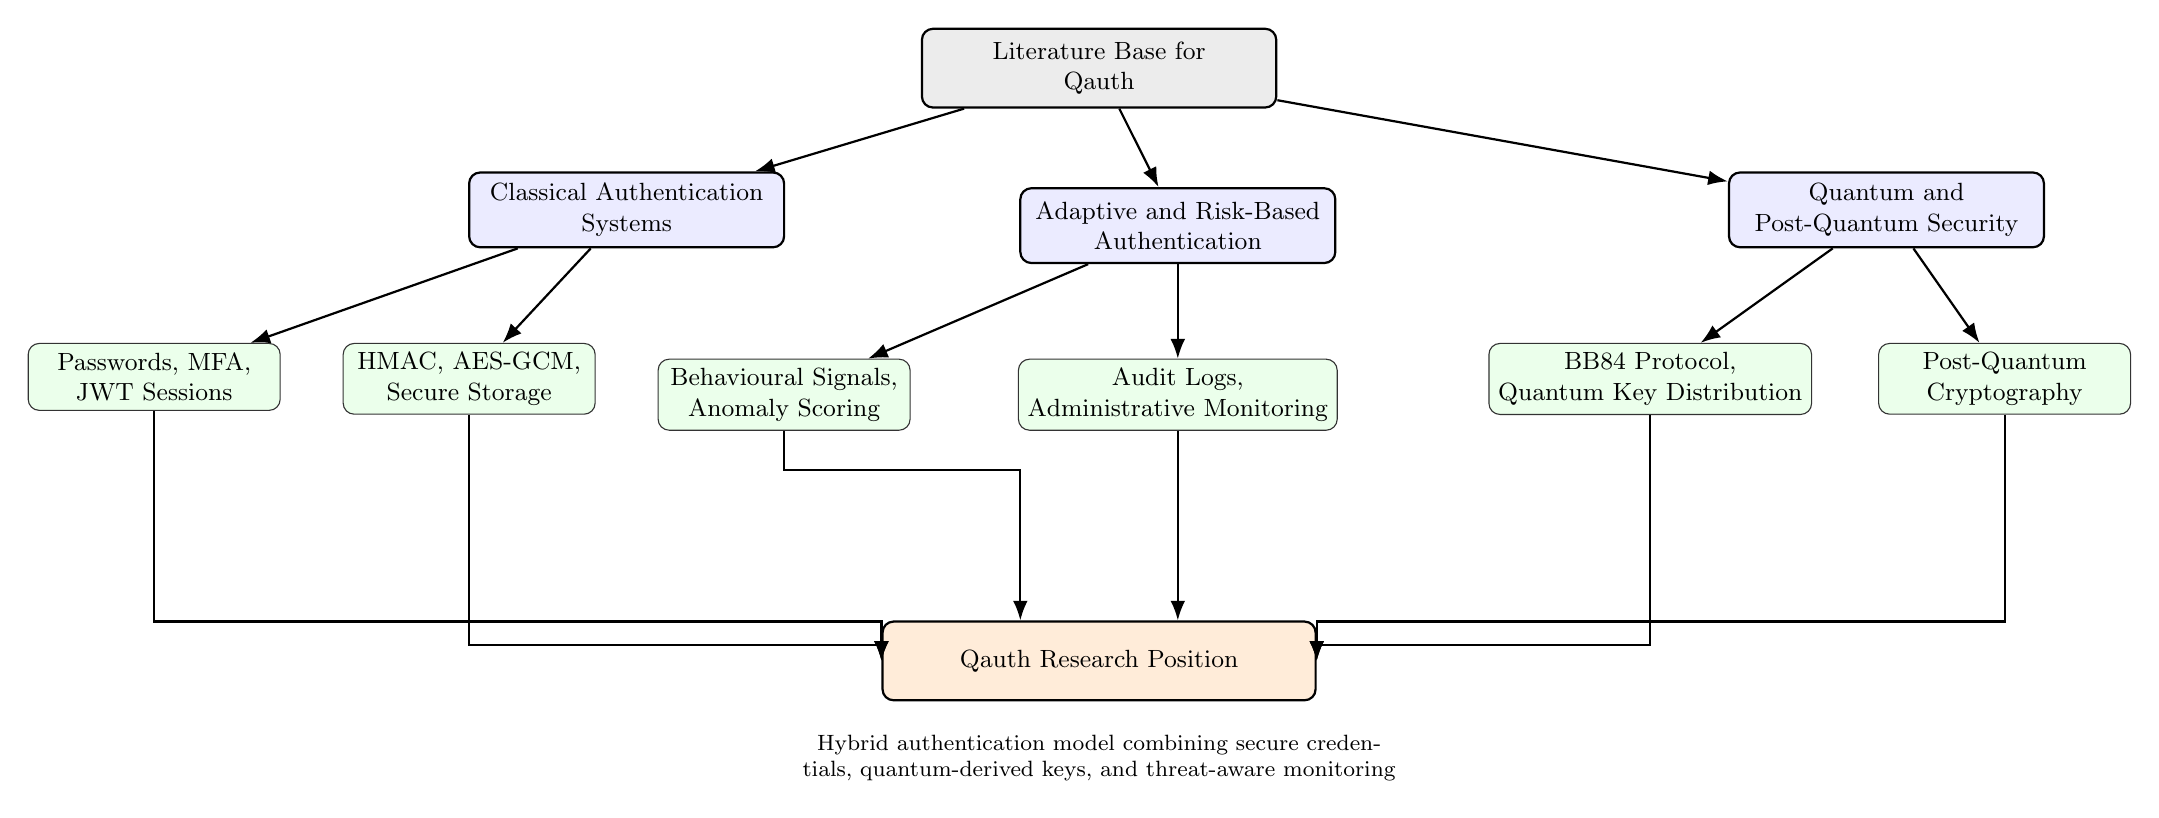
\begin{tikzpicture}[
  node distance=1.2cm and 0.5cm,
  every node/.style={align=center, font=\small},
  root/.style={rectangle, rounded corners, draw=black, thick, fill=gray!15, minimum width=4.5cm, minimum height=1cm},
  branch/.style={rectangle, rounded corners, draw=black, thick, fill=blue!8, minimum width=4cm, minimum height=0.95cm},
  leaf/.style={rectangle, rounded corners, draw=black!80, fill=green!8, minimum width=3.2cm, minimum height=0.85cm},
  arrow/.style={-{Latex[length=2.5mm]}, thick}
]

% --- CENTERED ROOT ---
\node[root] (core) at (-8, 0) {Literature Base for\\Qauth};

% --- FIRST LEVEL (Evenly Spaced) ---
\node[branch] (adaptive) at (-7, -2.0) {Adaptive and Risk-Based\\Authentication};
\node[branch] (classical) at (-14, -1.8) {Classical Authentication\\Systems};
\node[branch] (quantum) at (2, -1.8) {Quantum and\\Post-Quantum Security};

\draw[arrow] (core) -- (classical);
\draw[arrow] (core) -- (adaptive);
\draw[arrow] (core) -- (quantum);

% --- SECOND LEVEL (Leaves) ---
% Classical Leaves
\node[leaf, below=of classical, xshift=-6.0cm] (passwords) {Passwords, MFA,\\JWT Sessions};
\node[leaf, below=of classical, xshift=-2.0cm] (crypto) {HMAC, AES-GCM,\\Secure Storage};
\draw[arrow] (classical) -- (passwords);
\draw[arrow] (classical) -- (crypto);

% Adaptive Leaves
\node[leaf, below=of adaptive, xshift=-5.0cm] (anomaly) {Behavioural Signals,\\Anomaly Scoring};
\node[leaf, below=of adaptive, xshift=0cm] (monitoring) {Audit Logs,\\Administrative Monitoring};
\draw[arrow] (adaptive) -- (anomaly);
\draw[arrow] (adaptive) -- (monitoring);

% Quantum Leaves
\node[leaf, below=of quantum, xshift=-3.0cm] (bb84) {BB84 Protocol,\\Quantum Key Distribution};
\node[leaf, below=of quantum, xshift=1.5cm] (pqc) {Post-Quantum\\Cryptography};
\draw[arrow] (quantum) -- (bb84);
\draw[arrow] (quantum) -- (pqc);

% --- FINAL RESEARCH POSITION ---
\node[root, below=6.5cm of core, minimum width=5.5cm, fill=orange!15] (qauth) {Qauth Research Position};

% Connectors to Qauth
\draw[arrow] (passwords.south) |- ([yshift=0.5cm]qauth.west) -- (qauth.west);
\draw[arrow] (crypto.south) |- ([yshift=0.2cm]qauth.west) -- (qauth.west);
\draw[arrow] (anomaly.south) -- ++(0,-0.5) -| ([xshift=-1cm]qauth.north);
\draw[arrow] (monitoring.south) -- ++(0,-0.5) -| ([xshift=1cm]qauth.north);
\draw[arrow] (bb84.south) |- ([yshift=0.2cm]qauth.east) -- (qauth.east);
\draw[arrow] (pqc.south) |- ([yshift=0.5cm]qauth.east) -- (qauth.east);

\node[below=0.3cm of qauth, font=\footnotesize, text width=10cm] {Hybrid authentication model combining secure credentials, quantum-derived keys, and threat-aware monitoring};

\end{tikzpicture}
\end{adjustbox}
\caption{Literature map showing the conceptual relationship between classical authentication, adaptive security, and quantum-secured authentication in Qauth}
\label{fig:literature-map}
\end{figure}


\chapter{Proposed System}

\section{Introduction}
This chapter presents the design of Qauth as a layered authentication platform. The proposed system is not intended as a minimal login module; it is designed as an integrated security architecture in which authentication, quantum-derived key handling, login monitoring, and administrator visibility operate together. The design therefore emphasizes four properties: secure identity verification, controlled management of quantum key material, behavioural risk analysis, and auditability.

\section{Overview of Qauth}
Qauth is implemented as a full-stack web application composed of a React frontend, a Django REST backend, a PostgreSQL database, and a Redis-backed caching layer for transient counters used by the anomaly engine. The frontend provides public landing pages, login interactions, quantum verification feedback, and an administrator dashboard. The backend exposes APIs for registration, login, key management, challenge-response verification, event retrieval, and alert handling. The persistence layer stores users, encrypted key material, audit events, and threat alerts. The security engine is responsible for generating quantum-derived keys and scoring login behaviour.

The system can be understood as a sequence of trust-establishment layers:

\begin{enumerate}
    \item user identity is initially verified through credentials,
    \item a quantum-derived secret is associated with the user account,
    \item the secret is used in a challenge-response demonstration,
    \item the login attempt is scored for suspicious patterns,
    \item administrative interfaces expose system activity and threats.
\end{enumerate}

\section{Design Goals}
The proposed system is guided by the following design goals:

\begin{enumerate}
    \item \textbf{Security}: protect credentials, encrypt secret material, and identify suspicious access patterns.
    \item \textbf{Observability}: record all significant login events and expose them through administrative interfaces.
    \item \textbf{Layered Authentication}: combine static credential verification with quantum-derived key usage.
    \item \textbf{Controlled Secret Lifecycle}: support key generation, reveal restriction, fingerprinting, and rotation.
    \item \textbf{Extensibility}: allow future migration toward real quantum hardware or post-quantum cryptographic modules.
    \item \textbf{Educational Transparency}: make the internal security logic understandable and documentable.
\end{enumerate}

\section{System Requirements}

\subsection{Functional Requirements}
The main functional requirements of Qauth are as follows:

\begin{enumerate}
    \item The system shall allow a user to register with email, username, and password.
    \item The system shall create and store a quantum-derived key for the user.
    \item The system shall authenticate valid users through JWT-based login.
    \item The system shall support quantum-key reveal under a one-time-per-key policy.
    \item The system shall provide a challenge nonce for quantum login.
    \item The system shall verify an HMAC proof generated from the user's quantum key.
    \item The system shall record successful and failed login events.
    \item The system shall compute anomaly scores and risk levels for login attempts.
    \item The system shall expose monitoring endpoints for administrators.
    \item The system shall allow administrators to review and resolve threat alerts.
\end{enumerate}

\subsection{Non-Functional Requirements}
The important non-functional requirements are:

\begin{enumerate}
    \item \textbf{Confidentiality}: raw quantum keys must not be stored or transmitted in plaintext beyond controlled reveal operations.
    \item \textbf{Integrity}: authentication proofs and stored key records must be protected against tampering.
    \item \textbf{Availability}: authentication should continue even when external quantum randomness sources fail, through fallback generation.
    \item \textbf{Scalability}: stateless JWT sessions and Redis-backed counters support higher request volume than purely session-bound architectures.
    \item \textbf{Maintainability}: modular separation between authentication, quantum engine, and anomaly logic should simplify future extension.
    \item \textbf{Usability}: frontend flows should present verification progress clearly to end users and meaningful summaries to administrators.
\end{enumerate}

\section{High-Level Architecture}
% FIX: \noindent prevents double indent on first paragraph after section heading when indentfirst is active
\noindent The architecture of the proposed system can be summarised as follows:

% FIX: \noindent inside quote prevents double indentation (quote margin + parindent)
\begin{quote}
\noindent \textbf{Client Layer} $\rightarrow$ \textbf{React Frontend} $\rightarrow$ \textbf{Django REST API Layer} $\rightarrow$ \textbf{Authentication Module / Quantum Key Engine / Anomaly Engine} $\rightarrow$ \textbf{PostgreSQL and Redis}
\end{quote}

The frontend communicates with the backend over HTTP APIs. The backend enforces authentication, permission checks, request handling, key generation, challenge verification, and monitoring logic. PostgreSQL stores durable entities such as users, key metadata, login events, and alerts. Redis is used by the anomaly engine for short-lived counters and sets that represent behavioural patterns within a sliding time window.

\begin{figure}[H]
\centering
\begin{adjustbox}{max width=\textwidth, center}
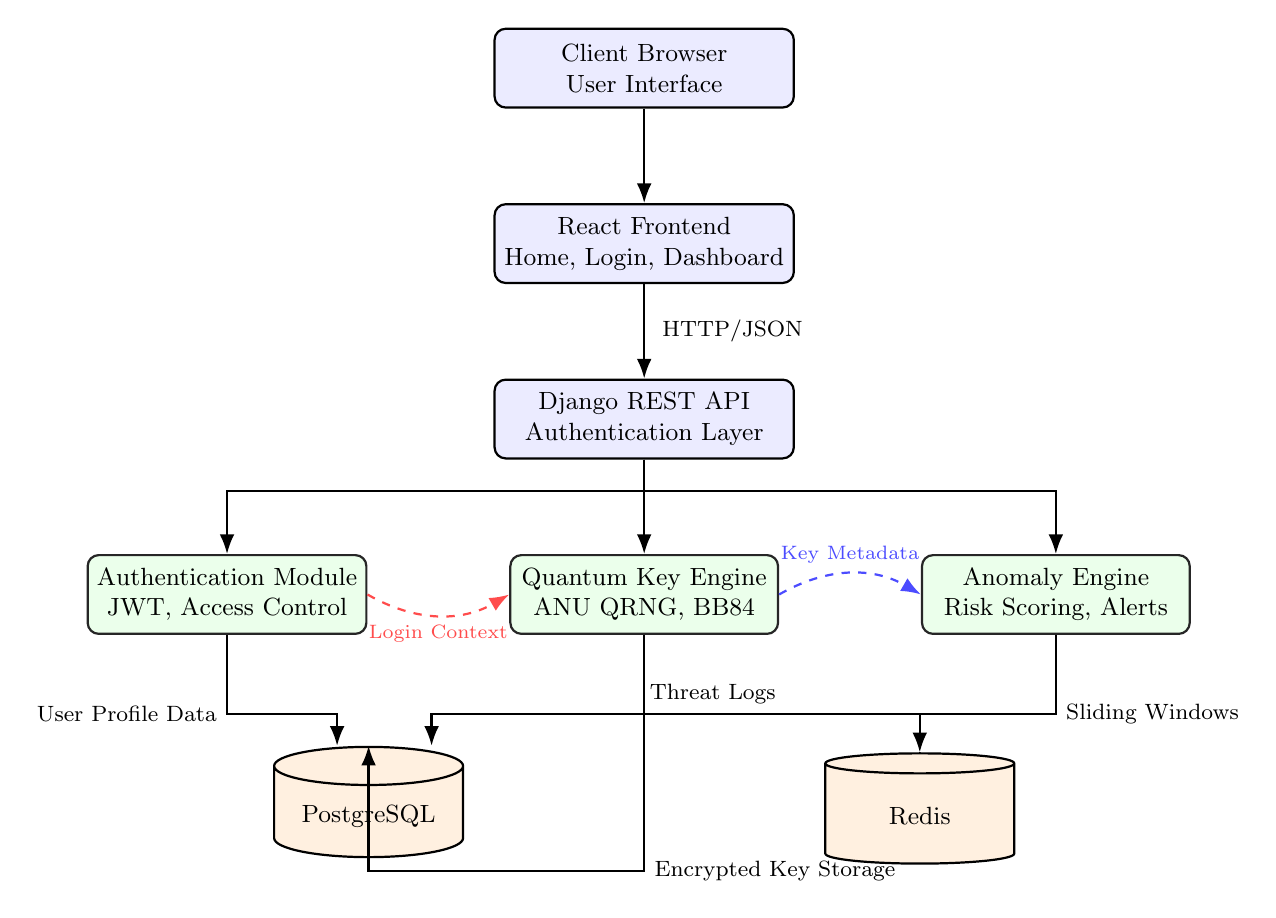
\begin{tikzpicture}[
  node distance=1.2cm and 1.2cm,
  every node/.style={align=center, font=\small},
  layer/.style={rectangle, rounded corners, draw=black, thick, minimum width=3.8cm, minimum height=1cm, fill=blue!8},
  service/.style={rectangle, rounded corners, draw=black!85, thick, minimum width=3.4cm, minimum height=1.0cm, fill=green!8},
  store/.style={cylinder, shape border rotate=90, aspect=0.25, draw=black, thick, minimum height=1.4cm, minimum width=2.4cm, fill=orange!12},
  arrow/.style={-{Latex[length=2.5mm]}, thick}
]

% --- VERTICAL STACK (Core Flow) ---
\node[layer] (client) {Client Browser\\User Interface};
\node[layer, below=of client] (frontend) {React Frontend\\Home, Login, Dashboard};
\node[layer, below=of frontend] (api) {Django REST API\\Authentication Layer};

% --- SERVICE LAYER (Horizontal Spread) ---
\node[service, below=of api] (quantum) {Quantum Key Engine\\ANU QRNG, BB84};
\node[service, left=1.8cm of quantum] (auth) {Authentication Module\\JWT, Access Control};
\node[service, right=1.8cm of quantum] (anomaly) {Anomaly Engine\\Risk Scoring, Alerts};

% --- DATABASE LAYER (Lowered to reduce congestion) ---
\node[store] (db) at (-3.5, -9.5) {PostgreSQL};
\node[store] (redis) at (3.5, -9.5) {Redis};

% --- TOP LEVEL FLOW ---
\draw[arrow] (client) -- (frontend);
\draw[arrow] (frontend) -- node[right, font=\footnotesize, xshift=0.1cm] {HTTP/JSON} (api);

% --- API TO SERVICES (Fan-out) ---
\draw[arrow] (api.south) -- ++(0,-0.4) -| (auth.north);
\draw[arrow] (api.south) -- (quantum.north);
\draw[arrow] (api.south) -- ++(0,-0.4) -| (anomaly.north);

% --- SERVICES TO DATABASE (Organized Routing) ---
% Auth to DB
\draw[arrow] (auth.south) -- ++(0,-1.0) -| ([xshift=-0.4cm]db.north) 
      node[pos=0, left, font=\footnotesize] {User Profile Data};

% Quantum to DB
\draw[arrow] (quantum.south) -- ++(0,-3.0) -| ([xshift=0cm]db.north) 
      node[pos=0, right, font=\footnotesize] {Encrypted Key Storage};

% Anomaly to DB
\draw[arrow] (anomaly.south) -- ++(0,-1.0) -| ([xshift=0.8cm]db.north) 
      node[pos=0.3, above, font=\footnotesize, xshift=0.4cm] {Threat Logs};

% Anomaly to Redis
\draw[arrow] (anomaly.south) -- ++(0,-1.0) -| (redis.north) 
      node[pos=0, right, font=\footnotesize] {Sliding Windows};

% --- INTER-SERVICE (Curved but offset) ---
\draw[arrow, dashed, blue!70] (quantum.east) to[out=30, in=150] 
      node[above, font=\scriptsize] {Key Metadata} (anomaly.west);
      
\draw[arrow, dashed, red!70] (auth.east) to[out=-30, in=210] 
      node[below, font=\scriptsize] {Login Context} (quantum.west);

\end{tikzpicture}
\end{adjustbox}
\caption{System architecture of Qauth with organized data flow and service interaction.}
\label{fig:qauth-architecture}
\end{figure}

\section{Core Modules of the System}

\subsection{Frontend Web Interface}
The frontend is implemented in React with routed pages for the home page, login flow, and administrator dashboard. The login page includes a quantum verification overlay that visualizes staged progress during credential validation, key access, nonce generation, proof computation, and session finalization. The dashboard displays login logs, key metadata, BB84 demonstration data, and risk analytics.

\subsection{Authentication Service}
The authentication service is implemented using Django REST Framework and SimpleJWT. It handles user registration, credential validation, token issuance, refresh logic, account lock checks, and endpoint-level authorization. A custom user model stores security-relevant metadata such as failed login counts and lock status.

\subsection{Quantum Key Engine}
The quantum key engine generates high-entropy secret material for each user. It attempts to obtain random bytes from the ANU Quantum Random Number Generator API. If the API is unavailable, it falls back to a BB84 simulation and then to the operating system cryptographic pseudo-random generator. The generated bytes are conditioned using SHA3-256 and stored in encrypted form.

\subsection{Login Anomaly Detection Engine}
The anomaly detection engine evaluates login requests using rule-based scoring. It considers repeated failures, request-rate behaviour, credential stuffing patterns, suspicious user-agent strings, locked accounts, and unusual login times. The engine produces a numeric score and a categorical risk level.

\subsection{Audit Logging and Threat Alert Module}
Every login attempt, successful or failed, is stored as a \texttt{LoginEvent}. The event contains network and behavioural context such as IP address, user agent, success state, failure reason, anomaly score, and triggered flags. High-risk behaviour can be escalated into \texttt{ThreatAlert} records that an administrator can review and resolve.

\subsection{Administrative Dashboard}
The administrative dashboard is designed for observability. It polls backend APIs for security metrics, login logs, risk distributions, key information, and demonstration endpoints. This supports real-time inspection of system behaviour and gives the project a monitoring dimension beyond ordinary login interfaces.

\section{User Roles and Access Control}
QAuth supports two broad user roles:

\begin{enumerate}
    \item \textbf{Standard user}: can register, authenticate, request quantum key metadata, perform key rotation, reveal a key once for demonstration, and complete quantum challenge-response login.
    \item \textbf{Administrator}: has all standard abilities and can additionally access statistics, login events, user lists, open alerts, and alert-resolution operations.
\end{enumerate}

Role separation is implemented through the \texttt{is\_admin} field in the custom user model and helper checks in protected backend views. This keeps privileged monitoring operations inaccessible to ordinary users.

\section{Authentication Workflows}

\subsection{Registration with Initial Quantum Key Provisioning}
During registration, the user submits email, username, password, and password confirmation. The backend validates password strength and matching confirmation using the registration serializer. A custom user is created, after which the quantum key engine generates and stores an encrypted quantum-derived key. The API returns user metadata and safe key metadata such as fingerprint and generation method.

\subsection{Credential-Based Login with Quantum Key Generation}
In the credential login flow, the backend validates email and password through the JWT serializer. On success, access and refresh tokens are issued. In the same flow, the system records the login attempt, computes anomaly scoring metadata, and ensures that the user's quantum key is generated or refreshed for the session context. This transforms login from a pure credential check into a session bootstrap event with security enrichment.

\subsection{Quantum Challenge-Response Login}
The quantum login flow is a second-stage authentication demonstration. The user first obtains the raw key through a one-time reveal endpoint, then requests a nonce from the backend. The frontend computes \texttt{HMAC-SHA256(nonce, quantum\_key)} using the Web Crypto API and sends the resulting proof to the backend. The backend recomputes the proof with the stored key and, if valid, issues JWT tokens. This process illustrates possession of user-specific secret material without resending the raw key.

\subsection{Quantum Key Rotation and One-Time Reveal Flow}
Qauth restricts key exposure through a one-time reveal model. Once a key is revealed, the corresponding record is marked with a reveal timestamp and cannot be revealed again. To obtain a new reveal, the user must rotate the key. This policy demonstrates controlled secret lifecycle management and limits repeated disclosure of raw key material.

\section{Threat Model and Security Assumptions}
The system assumes an adversary capable of attempting credential guessing, replaying requests, automating login attempts, and probing public endpoints with malicious user-agent patterns. The adversary is also assumed to exploit credential reuse or stolen passwords. The system addresses these risks through failure tracking, account locking, risk scoring, and audit logging.

At the same time, the project makes realistic prototype assumptions:

\begin{enumerate}
    \item the frontend runtime is trusted to compute HMAC proofs correctly for the user session,
    \item the backend environment securely stores the encryption secret used for protecting key material,
    \item the ANU QRNG service may be temporarily unavailable, requiring safe fallback logic,
    \item the BB84 implementation is a software simulation for educational and architectural purposes rather than a hardware QKD deployment.
\end{enumerate}

The threat model therefore balances realistic web security concerns with prototype constraints and makes clear what aspects of the system are demonstrative rather than production-certified.

\section{Advantages of the Proposed System}
Qauth offers several advantages compared with ordinary password-only authentication modules:

\begin{enumerate}
    \item it introduces high-entropy per-user secret material beyond the password,
    \item it secures stored key material using authenticated encryption,
    \item it supports a proof-based login demonstration using HMAC,
    \item it captures behavioural context for every login event,
    \item it provides administrative visibility into threats and anomalies,
    \item it remains operational through multi-level randomness fallback,
    \item it is designed in a modular way that supports future quantum-safe enhancements.
\end{enumerate}

\section{Summary}
The proposed Qauth system is a layered authentication architecture that combines user identity verification, quantum-derived key management, challenge-response proof validation, anomaly-aware login scoring, and administrator observability. It is designed to be secure, explainable, modular, and academically meaningful. The next chapter explains how this design is implemented in code, database structures, API endpoints, frontend flows, and deployment configuration.


\chapter{Methodology and Implementation}

\section{Introduction}
This chapter explains how Qauth is implemented in technical terms. The focus is on software architecture, database entities, cryptographic workflow, API design, and execution flow. Because the goal of the report is technical depth rather than superficial description, the chapter maps the document directly to the implemented code structure in the Django backend and React frontend.

\section{Development Methodology}
The project follows an iterative development methodology. The implementation began with the basic authentication skeleton, including user registration, credential login, and frontend routing. Once core authentication was functional, the quantum key pipeline was added as a service layer responsible for entropy acquisition, key derivation, storage encryption, and retrieval. The anomaly scoring engine was introduced next to make login attempts measurable and classifiable. Administrative endpoints and dashboard views were then added to expose observability. This staged approach reduced coupling and allowed each security layer to be validated independently before integration.

The methodology can be summarized in four implementation phases:

\begin{enumerate}
    \item base authentication and user lifecycle,
    \item quantum key generation and secure storage,
    \item challenge-response and login anomaly analysis,
    \item monitoring, dashboards, and system evaluation.
\end{enumerate}

\section{Technology Stack}

\subsection{Frontend Technologies}
The frontend is built using React and TypeScript. Client-side routing is handled with \texttt{react-router-dom}. The interface includes an animated landing page, a login page with quantum verification overlay, and an administrator dashboard that renders charts and API data views. Browser-native Web Crypto APIs are used for HMAC computation during the quantum login flow.

\subsection{Backend Technologies}
The backend is implemented in Django with Django REST Framework. JWT token support is provided by \texttt{djangorestframework-simplejwt}. Core authentication logic is exposed through REST endpoints, while view functions and serializers enforce validation, permission checks, and response shaping.

\subsection{Database and Persistence Layer}
The backend configuration uses PostgreSQL as the default relational database. Durable security records such as users, key metadata, login events, and threat alerts are stored in normalized relational tables. Short-lived counters used for anomaly analysis are stored in Redis through Django's caching framework.

\subsection{Cryptographic and Quantum Libraries}
The project uses the Python \texttt{cryptography} package for AES-GCM operations and key derivation support. Standard-library modules such as \texttt{hashlib}, \texttt{hmac}, \texttt{secrets}, and \texttt{urllib} are used for hash conditioning, challenge proof verification, randomness fallback, and external QRNG access. On the client side, HMAC computation is performed with the browser's \texttt{crypto.subtle} interface.

\section{Detailed System Architecture}

\subsection{Frontend Routing and Page Flow}
The React application defines three major routes: the home page (\texttt{/}), the login page (\texttt{/login}), and the administrative dashboard (\texttt{/dashboard}). This routing structure keeps user-facing onboarding, authentication, and administrative analytics separate. The login page implements the client-side stages of quantum verification, while the dashboard acts as both a monitoring interface and an API exploration utility.

\subsection{Backend Service Layer Design}
The backend uses separate modules for user authentication and security engines. The \texttt{authentication} app contains models, serializers, views, and URL routes for user operations and administrative security endpoints. The \texttt{engines} app contains the quantum key generation pipeline and anomaly scoring engine, as well as demo routes for direct experimentation. This separation improves maintainability by isolating security engines from user-facing request orchestration.

\subsection{Request Processing Pipeline}
The request pipeline typically follows this sequence:

\begin{enumerate}
    \item the frontend sends a request to an API endpoint,
    \item Django REST Framework applies authentication and permission checks,
    \item serializers validate request data where applicable,
    \item view functions coordinate model updates and engine execution,
    \item responses are returned as JSON payloads,
    \item frontend components update UI state based on the response.
\end{enumerate}

For login-related requests, the pipeline also includes behavioural scoring and audit event creation. This makes the pipeline security-aware rather than purely transactional.

\begin{figure}[H]
\centering
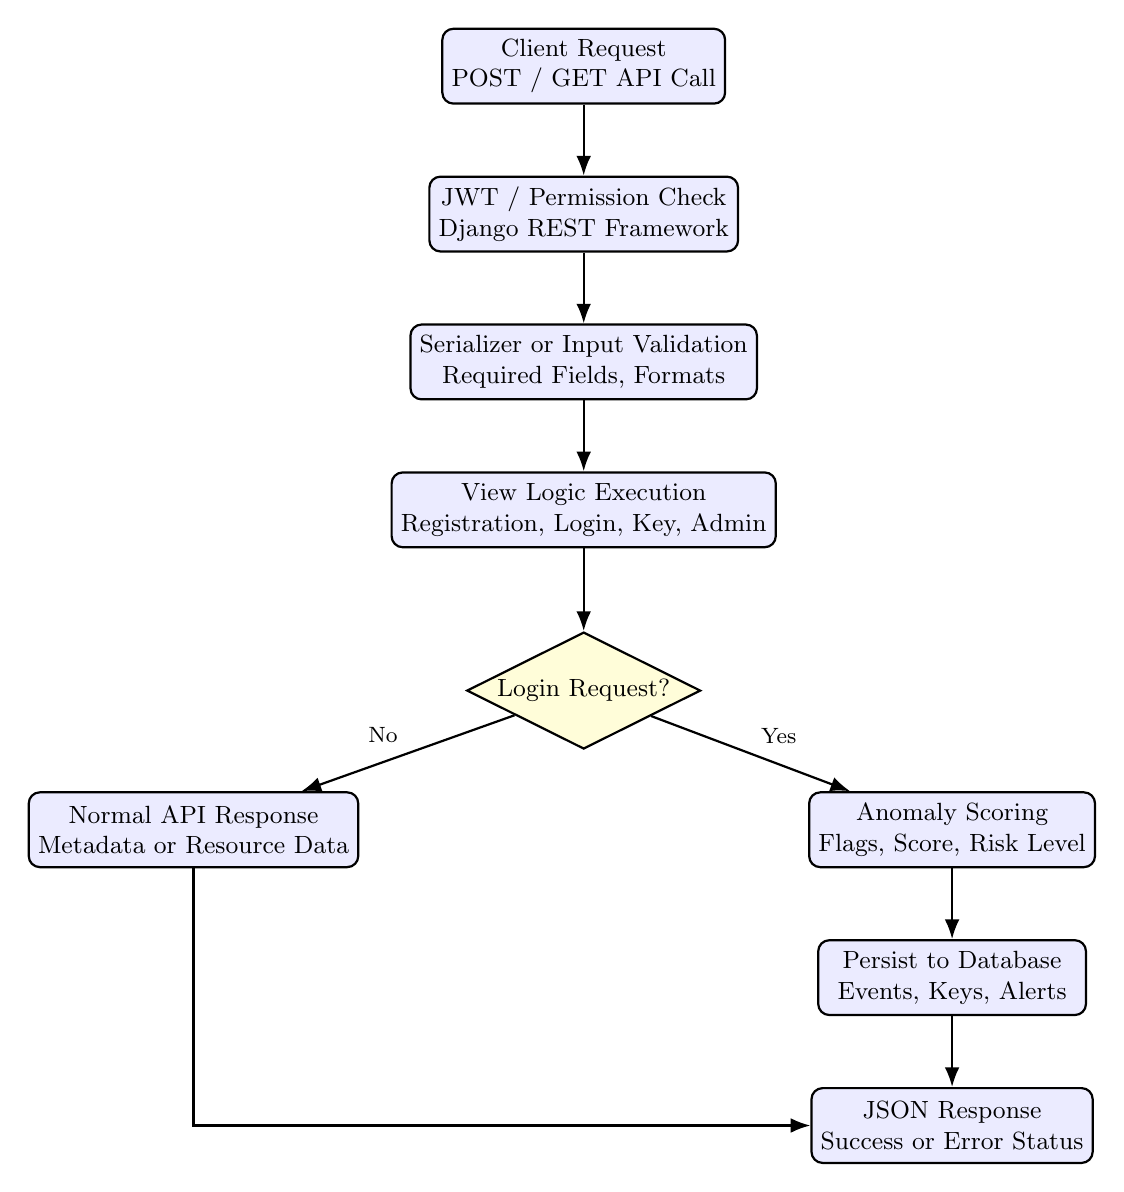
\begin{tikzpicture}[
  node distance=0.9cm and 1.0cm,
  every node/.style={align=center, font=\small},
  box/.style={rectangle, rounded corners, draw=black, thick, minimum width=3.4cm, minimum height=0.95cm, fill=blue!8},
  decision/.style={diamond, draw=black, thick, aspect=2.0, fill=yellow!15, inner sep=1pt},
  arrow/.style={-{Latex[length=2.5mm]}, thick}
]

\node[box] (request) {Client Request\\POST / GET API Call};
\node[box, below=of request] (authn) {JWT / Permission Check\\Django REST Framework};
\node[box, below=of authn] (validate) {Serializer or Input Validation\\Required Fields, Formats};
\node[box, below=of validate] (logic) {View Logic Execution\\Registration, Login, Key, Admin};
\node[decision, below=of logic, yshift=-0.15cm] (risk) {Login Request?};
\node[box, below left=of risk, xshift=-1.1cm] (normal) {Normal API Response\\Metadata or Resource Data};
\node[box, below right=of risk, xshift=1.1cm] (score) {Anomaly Scoring\\Flags, Score, Risk Level};
\node[box, below=of score] (persist) {Persist to Database\\Events, Keys, Alerts};
\node[box, below=of persist] (response) {JSON Response\\Success or Error Status};

\draw[arrow] (request) -- (authn);
\draw[arrow] (authn) -- (validate);
\draw[arrow] (validate) -- (logic);
\draw[arrow] (logic) -- (risk);
\draw[arrow] (risk) -- node[above left, font=\footnotesize] {No} (normal);
\draw[arrow] (risk) -- node[above right, font=\footnotesize] {Yes} (score);
\draw[arrow] (normal.south) |- (response.west);
\draw[arrow] (score) -- (persist);
\draw[arrow] (persist) -- (response);

\end{tikzpicture}
\caption{API workflow of Qauth showing request validation, authentication checks, application logic, anomaly scoring, persistence, and JSON response generation}
\label{fig:api-workflow}
\end{figure}

\section{Database Design}

\subsection{Entity Relationship Overview}
The database model of Qauth is centered on the custom user account. Each user can own one quantum key record and can produce multiple login events. Each login event can, in turn, be associated with one or more threat alerts. The relational structure is therefore:

% FIX: \noindent inside quote prevents double indentation (quote margin + parindent)
\begin{quote}
\noindent \texttt{QAuthUser} $\rightarrow$ \texttt{QuantumKey} (one-to-one) \\
\texttt{QAuthUser} $\rightarrow$ \texttt{LoginEvent} (one-to-many) \\
\texttt{LoginEvent} $\rightarrow$ \texttt{ThreatAlert} (one-to-many)
\end{quote}

\begin{figure}[H]
\centering
\begin{adjustbox}{max width=\textwidth, center}
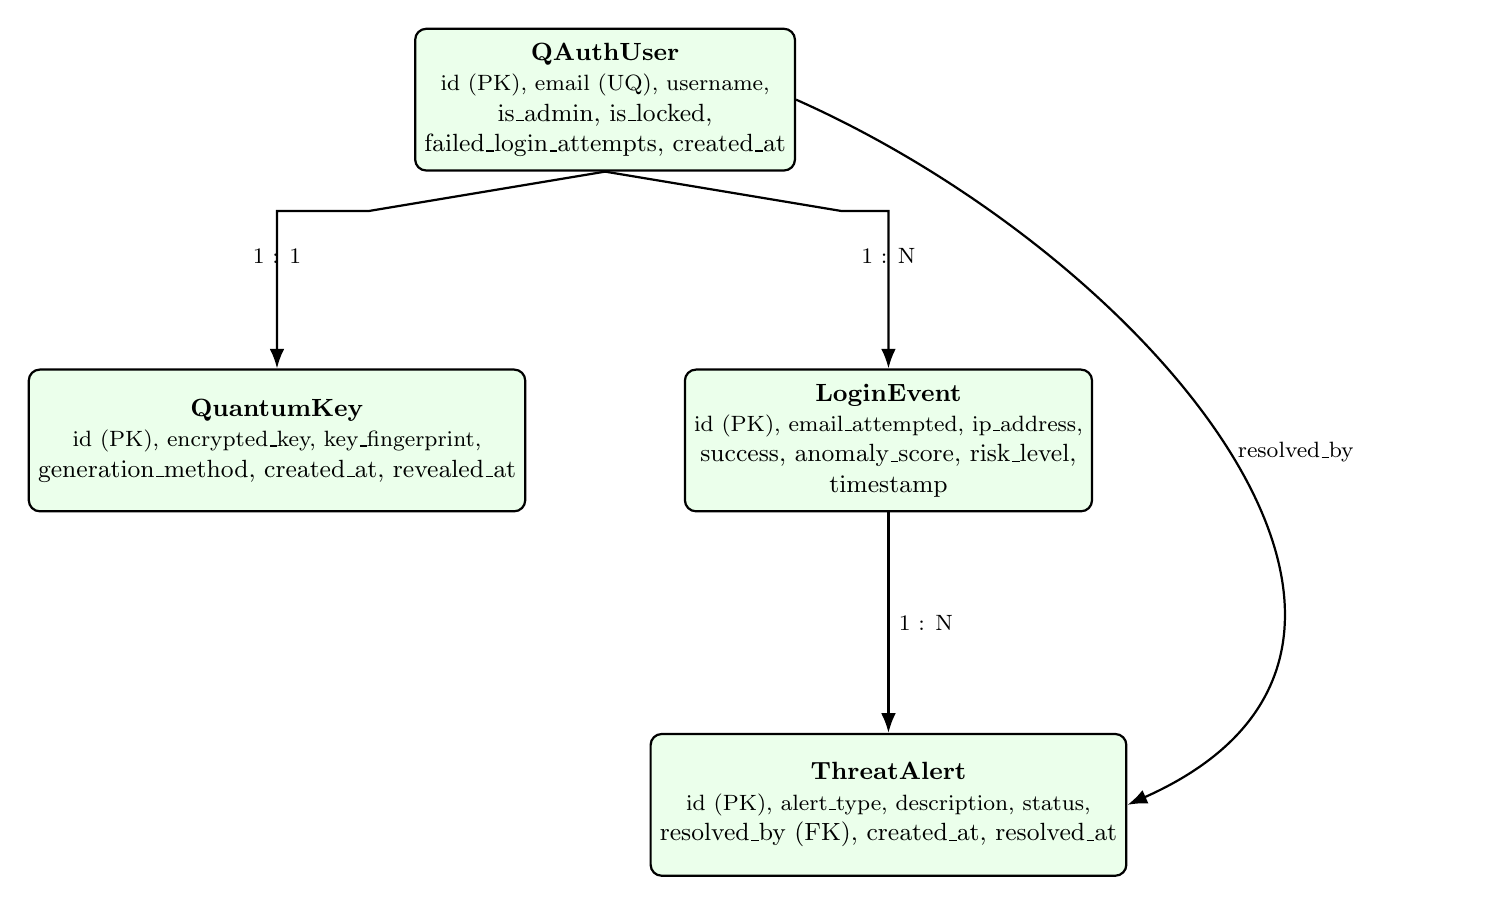
\begin{tikzpicture}[
  % Increased vertical node distance to 2.8cm
  node distance=2.8cm and 2.5cm,
  every node/.style={align=center, font=\small},
  entity/.style={rectangle, draw=black, thick, rounded corners, minimum width=4.8cm, minimum height=1.8cm, fill=green!8},
  arrow/.style={-{Latex[length=2.5mm]}, thick}
]

% --- CENTERED ROOT ---
\node[entity] (user) {\textbf{QAuthUser}\\
\footnotesize id (PK), email (UQ), username,\\ is\_admin, is\_locked,\\ failed\_login\_attempts, created\_at};

% --- SYMMETRICAL MIDDLE LAYER ---
\node[entity, below left=2.5cm and 1.0cm of user.south] (qkey) {\textbf{QuantumKey}\\
\footnotesize id (PK), encrypted\_key, key\_fingerprint,\\ generation\_method, created\_at, revealed\_at};

\node[entity, below right=2.5cm and 1.0cm of user.south] (event) {\textbf{LoginEvent}\\
\footnotesize id (PK), email\_attempted, ip\_address,\\ success, anomaly\_score, risk\_level,\\ timestamp};

% --- BOTTOM LAYER ---
\node[entity, below=2.8cm of event] (alert) {\textbf{ThreatAlert}\\
\footnotesize id (PK), alert\_type, description, status,\\ resolved\_by (FK), created\_at, resolved\_at};

% --- RELATIONSHIP CONNECTORS ---
\draw[arrow] (user.south) -- ++(-3.0,-0.5) -| (qkey.north) 
      node[pos=0.7, above, font=\footnotesize] {1 : 1};

\draw[arrow] (user.south) -- ++(3.0,-0.5) -| (event.north) 
      node[pos=0.7, above, font=\footnotesize] {1 : N};

\draw[arrow] (event.south) -- (alert.north) 
      node[midway, right, font=\footnotesize] {1 : N};

\draw[arrow] (user.east) .. controls +(4.5,-2.0) and +(4.5,2.0) .. 
      node[right, font=\footnotesize] {resolved\_by} (alert.east);

\end{tikzpicture}
\end{adjustbox}
\caption{Expanded ER diagram of the Qauth database.}
\label{fig:er-diagram}
\end{figure}

\subsection{QAuthUser Table Schema}
The \texttt{QAuthUser} model extends Django's \texttt{AbstractBaseUser} and \texttt{PermissionsMixin}. It serves as the central identity record for the system.

\begin{table}[H]
\centering
\small
\renewcommand{\arraystretch}{1.3}
\caption{Schema of \texttt{qauth\_users}}
\label{tab:qauth-users}
\begin{tabular}{|p{4.0cm}|p{2.8cm}|p{1.8cm}|p{5.5cm}|}
\hline
\textbf{Field} & \textbf{Type} & \textbf{Constraint} & \textbf{Purpose} \\
\hline
\texttt{id} & UUID & Primary key & Unique identifier for each user \\
\hline
\texttt{email} & EmailField & Unique & Primary login identity \\
\hline
\texttt{username} & CharField & Unique & Human-readable user identifier \\
\hline
\texttt{is\_active} & Boolean & Default True & Indicates account activity \\
\hline
\texttt{is\_staff} & Boolean & Default False & Django administrative flag \\
\hline
\texttt{is\_admin} & Boolean & Default False & Qauth administrative access flag \\
\hline
\texttt{is\_locked} & Boolean & Default False & Indicates lock due to failed attempts \\
\hline
\texttt{failed\_login\_attempts} & PositiveInteger & Default 0 & Counter for brute-force tracking \\
\hline
\texttt{last\_failed\_login} & DateTime & Nullable & Timestamp of last failed attempt \\
\hline
\texttt{quantum\_key\_id} & CharField & Nullable & Reference identifier for quantum key metadata \\
\hline
\texttt{created\_at} & DateTime & Default now & Record creation timestamp \\
\hline
\texttt{updated\_at} & DateTime & Auto-updated & Last modification timestamp \\
\hline
\end{tabular}
\end{table}

The model also contains utility methods to increment failed attempts and reset account state. Once the failure count reaches the threshold of five, the account is locked.

\subsection{QuantumKey Table Schema}
The \texttt{QuantumKey} model stores key metadata and encrypted secret material.

\begin{table}[H]
\centering
\small
\caption{Schema of \texttt{quantum\_keys}}
\label{tab:quantum-keys}
\begin{tabular}{|p{3.0cm}|p{2.8cm}|p{1.8cm}|p{6.0cm}|}
\hline
\textbf{Field} & \textbf{Type} & \textbf{Constraint} & \textbf{Purpose} \\
\hline
\texttt{id} & UUID & Primary key & Unique key record identifier \\
\hline
\texttt{user} & OneToOneField & Unique relation & Associates one key with one user \\
\hline
\texttt{encrypted\_key} & BinaryField & Required & AES-GCM ciphertext of conditioned key \\
\hline
\texttt{key\_fingerprint} & CharField & Required & SHA-256 fingerprint for safe identification \\
\hline
\texttt{generation\_method} & CharField & Choice field & Indicates \texttt{qrng\_api}, \texttt{bb84\_sim}, or \texttt{fallback} \\
\hline
\texttt{created\_at} & DateTime & Default now & Timestamp of key creation \\
\hline
\texttt{rotated\_at} & DateTime & Nullable & Timestamp of latest rotation \\
\hline
\texttt{revealed\_at} & DateTime & Nullable & Used to enforce one-time reveal policy \\
\hline
\end{tabular}
\end{table}

\subsection{LoginEvent Table Schema}
The \texttt{LoginEvent} model functions as an audit trail and security telemetry record.

\begin{table}[H]
\centering
\small
\caption{Schema of \texttt{login\_events}}
\label{tab:login-events}
\begin{tabular}{|p{3.0cm}|p{2.8cm}|p{1.8cm}|p{6.0cm}|}
\hline
\textbf{Field} & \textbf{Type} & \textbf{Constraint} & \textbf{Purpose} \\
\hline
\texttt{id} & UUID & Primary key & Unique event identifier \\
\hline
\texttt{user} & ForeignKey & Nullable & Associated user, if known \\
\hline
\texttt{email\_attempted} & EmailField & Required & Email involved in the attempt \\
\hline
\texttt{ip\_address} & IP field & Required & Source IP of the request \\
\hline
\texttt{user\_agent} & TextField & Optional & Client user-agent string \\
\hline
\texttt{success} & Boolean & Required & Whether authentication succeeded \\
\hline
\texttt{failure\_reason} & CharField & Optional & Short explanation for failure \\
\hline
\texttt{anomaly\_score} & FloatField & Default 0.0 & Composite security score \\
\hline
\texttt{risk\_level} & CharField & Choice field & \texttt{low}, \texttt{medium}, \texttt{high}, or \texttt{critical} \\
\hline
\texttt{anomaly\_flags} & JSONField & Default list & Triggered anomaly rule labels \\
\hline
\texttt{timestamp} & DateTime & Default now & Event occurrence time \\
\hline
\end{tabular}
\end{table}

\subsection{ThreatAlert Table Schema}
The \texttt{ThreatAlert} model stores escalated security conditions.

\begin{table}[H]
\centering
\small
\caption{Schema of \texttt{threat\_alerts}}
\label{tab:threat-alerts}
\begin{tabular}{|p{3.0cm}|p{2.8cm}|p{1.8cm}|p{6.0cm}|}
\hline
\textbf{Field} & \textbf{Type} & \textbf{Constraint} & \textbf{Purpose} \\
\hline
\texttt{id} & UUID & Primary key & Unique alert identifier \\
\hline
\texttt{login\_event} & ForeignKey & Required & Source event for the alert \\
\hline
\texttt{alert\_type} & CharField & Choice field & Nature of the threat \\
\hline
\texttt{description} & TextField & Required & Human-readable explanation \\
\hline
\texttt{status} & CharField & Default open & Workflow state of the alert \\
\hline
\texttt{resolved\_by} & ForeignKey & Nullable & Administrator who resolved it \\
\hline
\texttt{created\_at} & DateTime & Default now & Creation timestamp \\
\hline
\texttt{resolved\_at} & DateTime & Nullable & Resolution timestamp \\
\hline
\end{tabular}
\end{table}

\subsection{Indexing and Data Integrity Constraints}
The \texttt{LoginEvent} model defines indexes on \texttt{ip\_address + timestamp}, \texttt{user + timestamp}, and \texttt{risk\_level}. These indexes improve the efficiency of administrative filtering by IP, user, and risk class. Integrity is also enforced through unique constraints on email and username in the user table, and the one-to-one relation between user and key.

\section{Implementation of the Authentication Module}

\subsection{Custom User Manager and User Model Logic}
The custom user manager provides two main creation methods: \texttt{create\_user} and \texttt{create\_superuser}. The first normalizes email input, hashes the password using Django's built-in secure password handling, and stores the record. The second sets elevated privilege flags. This design ensures that identity records remain compatible with Django authentication while also supporting Qauth-specific fields such as quantum-key linkage and lock state.

The \texttt{increment\_failed\_attempts()} method is security critical. Every failed attempt increments a counter, records the timestamp, and locks the account after five failures. This creates a local account-based defence layer in addition to IP-based anomaly scoring.

\subsection{Registration Serializer and User Creation Flow}
The registration serializer accepts \texttt{email}, \texttt{username}, \texttt{password}, and \texttt{password2}. The validation logic explicitly compares the two password fields and raises a serializer error if they differ. On successful validation, the serializer delegates user creation to the custom user manager. The registration view then generates an initial quantum key and returns user-safe metadata.

\subsection{JWT Token Issuance and Session Handling}
JWT issuance is handled through a custom serializer derived from \texttt{TokenObtainPairSerializer}. This approach allows Qauth to preserve the normal access/refresh token workflow while injecting additional behaviour. After successful authentication, the serializer records a login event, calculates risk metadata, and triggers key generation. This is a strong design decision because it keeps session bootstrap and security telemetry synchronized in one place.

\subsection{Failed Login Tracking and Account Locking}
When authentication fails, the serializer catches the failure path and records the event without blocking the natural error response. If the target email belongs to an existing account, the user model counter is incremented and the anomaly engine is called. The backend therefore captures failure telemetry even when the authentication transaction itself is rejected.

\section{Implementation of the Quantum Key Engine}

\subsection{BB84 Simulation Logic}
The BB84 simulator models the following steps: Alice generates random bits and random bases, Bob measures them using his own random bases, matching-basis positions are sifted, a subset is sampled to estimate quantum bit error rate (QBER), and the remaining bits are compressed into a privacy-amplified key using SHA3-256. The simulation also tracks whether the estimated QBER crosses an abort threshold associated with eavesdropper suspicion. Although this is a software simulation rather than a physical QKD channel, it accurately captures the educational logic of basis mismatch, measurement uncertainty, and error-rate inspection.

\subsection{ANU QRNG API Integration}
The preferred randomness source is the ANU Quantum Random Number Generator API. The engine requests unsigned byte values over HTTP and validates that the response contains sufficient data. If the service is available, the returned bytes become the basis for the conditioned key. This layer gives the system an authentic quantum randomness source when network conditions permit.

\subsection{Fallback Randomness Strategy}
A key architectural strength of Qauth is that it does not depend on a single randomness source. If the external QRNG call fails, the system attempts BB84 simulation. If that also fails, it falls back to \texttt{secrets.token\_bytes()}, which uses the operating system cryptographically secure random generator. This three-level strategy improves availability and ensures the authentication workflow is not blocked by external entropy failures.

\subsection{SHA3-256 Key Conditioning}
Once raw random bytes are obtained, they are passed through SHA3-256. The purpose of this step is to normalize the output into a fixed-length, well-conditioned hex key. It also creates a deterministic final representation independent of the randomness source. This conditioned output then becomes the logical quantum-derived key used by the rest of the platform.

\subsection{AES-256-GCM Encryption of Stored Keys}
Raw key material is never stored directly in plaintext. The key manager encrypts the conditioned key using AES-256-GCM before persistence. AES-GCM is an authenticated encryption mode that simultaneously ensures confidentiality and integrity. This choice is appropriate for stored secret material because it reduces the risk that a database compromise would expose directly usable quantum keys.

\subsection{Key Fingerprinting and Metadata Management}
In addition to the encrypted key, the system stores a fingerprint generated from a SHA-256 digest of the plaintext key. The fingerprint is not sufficient to recover the original key, but it is useful for safe identification in responses, dashboards, and audit contexts. Metadata such as generation method, creation timestamp, rotation timestamp, and reveal timestamp complete the key lifecycle record.

\subsection{Quantum Key Reveal and Rotation Mechanisms}
The \texttt{quantum-key-reveal} endpoint returns the raw key only if the key has not yet been revealed. After a successful reveal, the backend sets \texttt{revealed\_at}, preventing further disclosure of the same key. The \texttt{rotate-key} endpoint generates a fresh key and updates metadata so the one-time reveal cycle can repeat. This approach demonstrates controlled exposure and forward movement of key state.

\section{Implementation of the Login Anomaly Detection Engine}

\subsection{Rule-Based Risk Scoring Model}
The anomaly scoring engine computes a composite score from six rule families: brute-force activity, IP request rate, credential stuffing, bot-like user-agent patterns, locked account targeting, and unusual time-of-day access. Each rule contributes a weighted amount to the total score, and the sum is capped at 1.0. The score is then mapped into a categorical level: \texttt{low}, \texttt{medium}, \texttt{high}, or \texttt{critical}.

\subsection{Sliding Window Counters}
The engine uses Redis-backed cache entries with a 300-second lifetime to maintain counters and sets across short windows. This enables the system to recognize patterns that individual requests cannot reveal, such as repeated attempts from the same IP or many distinct emails targeted by one source. The design is lightweight and suitable for near-real-time risk analysis.

\subsection{Bot Pattern Detection}
The engine checks the user-agent string against known automation markers such as \texttt{curl}, \texttt{wget}, and \texttt{python-requests}. Empty user-agent strings are also treated as suspicious. This rule is especially useful because many scripted attacks expose recognizable HTTP fingerprints even when credentials themselves appear syntactically valid.

\subsection{Credential Stuffing Detection}
Credential stuffing is inferred by tracking the number of distinct email identities attempted from the same IP within the time window. This is operationally different from brute-force attacks on a single account. By separating these patterns, Qauth produces more informative flags for administrators.

\subsection{Time-Based Anomaly Detection}
The time anomaly rule marks logins occurring during an unusual UTC time band between 02:00 and 05:00. Although this is a simplified heuristic, it demonstrates how temporal context can be included in risk evaluation. In future systems, this rule could be personalized per user rather than fixed globally.

\subsection{Composite Risk Score and Risk Level Mapping}
The final score is translated using thresholds: 0.00--0.25 is low, 0.25--0.55 is medium, 0.55--0.80 is high, and 0.80 or above is critical. This categorical mapping simplifies dashboard representation and administrative action. It also creates a bridge between low-level counters and human-readable threat language.

\section{API Design and Endpoint Specification}
Qauth exposes its main application logic through REST endpoints under \texttt{/api/auth/} and supporting demo endpoints under \texttt{/api/quantum/}. Table \ref{tab:api-endpoints} summarizes the major routes.

\begin{table}[H]
\centering
\scriptsize
\caption{Major API endpoints in Qauth}
\label{tab:api-endpoints}
\begin{tabular}{|p{4.5cm}|p{1.2cm}|p{2.0cm}|p{6.5cm}|}
\hline
\textbf{Endpoint} & \textbf{Method} & \textbf{Access} & \textbf{Purpose} \\
\hline
\texttt{/api/auth/register/} & POST & Public & Create user and provision initial quantum key \\
\hline
\texttt{/api/auth/token/} & POST & Public & Validate credentials and issue JWT pair \\
\hline
\texttt{/api/auth/token/refresh/} & POST & Public & Refresh JWT access token \\
\hline
\texttt{/api/auth/rotate-key/} & POST & Authenticated & Rotate the current user's quantum key \\
\hline
\texttt{/api/auth/quantum-key-reveal/} & GET & Authenticated & Reveal raw key once for the current key record \\
\hline
\texttt{/api/auth/quantum-challenge/} & POST & Public & Return nonce for challenge-response flow \\
\hline
\texttt{/api/auth/quantum-login/} & POST & Public & Validate HMAC proof and issue JWT pair \\
\hline
\texttt{/api/auth/key-info/} & GET & Authenticated & Return safe key metadata for current user \\
\hline
\texttt{/api/auth/bb84-demo/} & GET & Public & Return BB84 protocol statistics without key exposure \\
\hline
\texttt{/api/auth/stats/} & GET & Admin & Return security summary metrics \\
\hline
\texttt{/api/auth/events/} & GET & Admin & Return filtered login event list \\
\hline
\texttt{/api/auth/alerts/} & GET & Admin & Return open or investigating alerts \\
\hline
\texttt{/api/auth/alerts/\{alert\_id\}\allowbreak/resolve/} & PATCH & Admin & Update alert status and resolver metadata \\
\hline
\texttt{/api/auth/users/} & GET & Admin & Return user list and security state \\
\hline
\texttt{/api/quantum/quantum-key-demo/} & GET & Public & Demo metadata for quantum key generation pipeline \\
\hline
\texttt{/api/quantum/anomaly-score-demo/} & GET & Public & Demo scoring result for supplied inputs \\
\hline
\end{tabular}
\end{table}

\subsection{Authentication Endpoints}
The authentication endpoints cover user registration, credential login, token refresh, and user-specific key metadata operations. Their purpose is to establish authenticated application sessions and manage user security state.

\subsection{Quantum Security Endpoints}
The quantum security endpoints cover reveal, challenge issuance, challenge-response login, key rotation, and BB84 demonstration. These endpoints are the distinguishing feature of Qauth and express the platform's quantum-aware design.

\subsection{Administrative Monitoring Endpoints}
Administrative endpoints provide aggregate metrics, filtered event logs, alert lists, alert resolution, and user overviews. They turn the backend into an observable security service rather than a black-box authenticator.

\subsection{Request and Response Payload Structures}
Selected request structures are summarized below:

\begin{table}[H]
\centering
\small
\caption{Representative request payloads}
\label{tab:payloads}
\begin{tabular}{|p{3.6cm}|p{8.8cm}|}
\hline
\textbf{Operation} & \textbf{Important fields} \\
\hline
Registration & \texttt{email}, \texttt{username}, \texttt{password}, \texttt{password2} \\
\hline
Credential login & \texttt{email}, \texttt{password} \\
\hline
Quantum challenge request & \texttt{email} \\
\hline
Quantum login & \texttt{email}, \texttt{nonce}, \texttt{proof} \\
\hline
Resolve alert & \texttt{status} where status is one of resolved, false\_positive, or investigating \\
\hline
\end{tabular}
\end{table}

\subsection{Error Handling Strategy}
The backend consistently returns JSON errors with HTTP status codes appropriate to missing data, forbidden access, failed proof verification, or unresolved resources. Important examples include 400 for missing fields, 401 for invalid proofs, 403 for unauthorized administrative access or repeated key reveal, and 404 for nonexistent records. This makes the API predictable and easier to integrate into frontend state handling.

\section{Sequence Diagrams}

\begin{figure}[H]
\centering
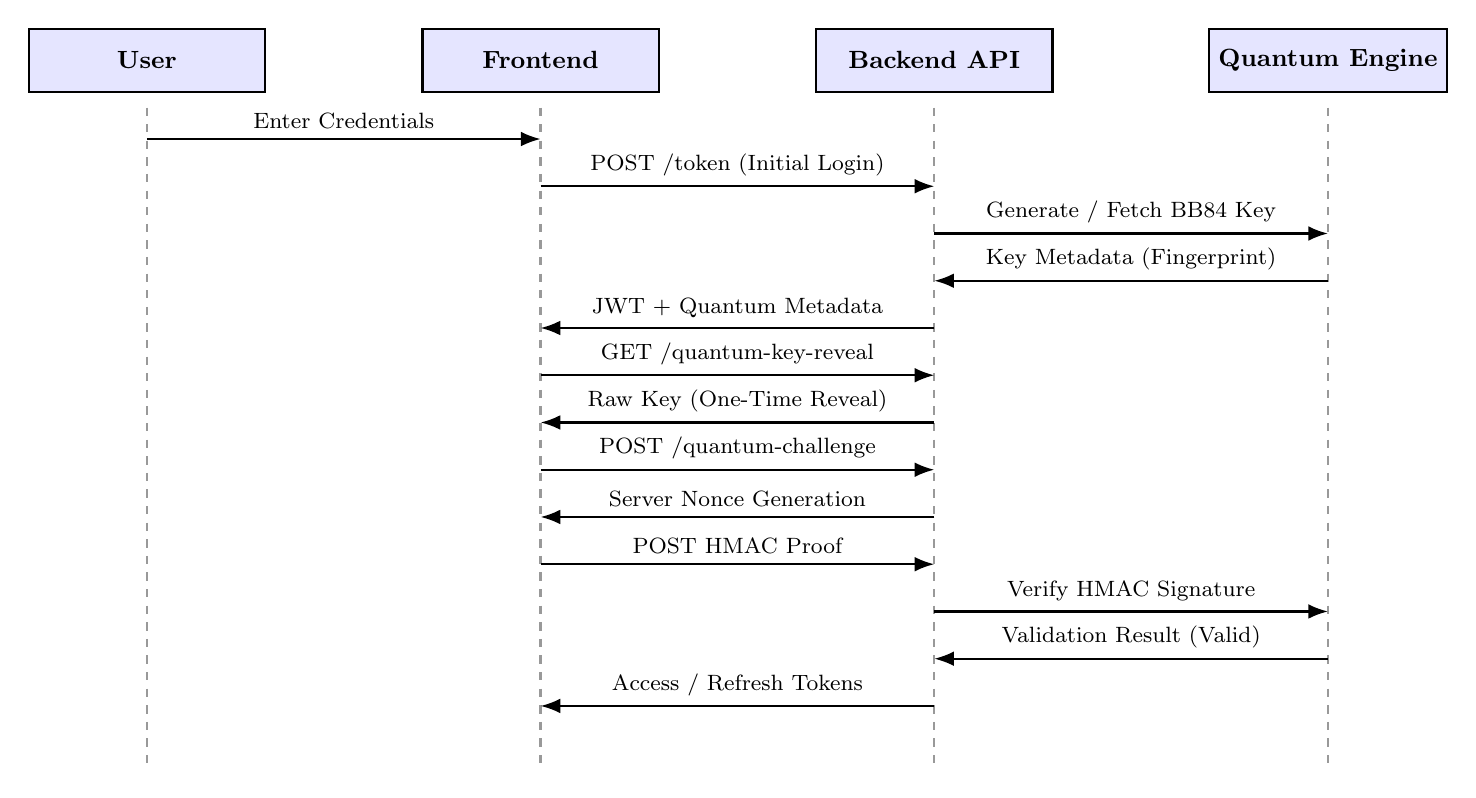
\begin{tikzpicture}[
  every node/.style={font=\small, align=center},
  lifeline/.style={draw=black, thick, dashed, opacity=0.4},
  header/.style={rectangle, draw, thick, fill=blue!10, minimum width=3cm, minimum height=0.8cm},
  arrow/.style={-{Latex[length=2.5mm]}, thick}
]

\def\colspacing{5.0}

\coordinate (C1) at (0,0);
\coordinate (C2) at (\colspacing,0);
\coordinate (C3) at (2*\colspacing,0);
\coordinate (C4) at (3*\colspacing,0);

\node[header] (user) at (C1) {\textbf{User}};
\node[header] (front) at (C2) {\textbf{Frontend}};
\node[header] (api) at (C3) {\textbf{Backend API}};
\node[header] (engine) at (C4) {\textbf{Quantum Engine}};

\draw[lifeline] (C1) ++(0,-0.6) -- ++(0,-8.4);
\draw[lifeline] (C2) ++(0,-0.6) -- ++(0,-8.4);
\draw[lifeline] (C3) ++(0,-0.6) -- ++(0,-8.4);
\draw[lifeline] (C4) ++(0,-0.6) -- ++(0,-8.4);

\draw[arrow] (0,-1.0) -- node[above, font=\footnotesize] {Enter Credentials} (\colspacing,-1.0);
\draw[arrow] (\colspacing,-1.6) -- node[above, font=\footnotesize] {POST /token (Initial Login)} (2*\colspacing,-1.6);
\draw[arrow] (2*\colspacing,-2.2) -- node[above, font=\footnotesize] {Generate / Fetch BB84 Key} (3*\colspacing,-2.2);
\draw[arrow] (3*\colspacing,-2.8) -- node[above, font=\footnotesize] {Key Metadata (Fingerprint)} (2*\colspacing,-2.8);
\draw[arrow] (2*\colspacing,-3.4) -- node[above, font=\footnotesize] {JWT + Quantum Metadata} (\colspacing,-3.4);
\draw[arrow] (\colspacing,-4.0) -- node[above, font=\footnotesize] {GET /quantum-key-reveal} (2*\colspacing,-4.0);
\draw[arrow] (2*\colspacing,-4.6) -- node[above, font=\footnotesize] {Raw Key (One-Time Reveal)} (\colspacing,-4.6);
\draw[arrow] (\colspacing,-5.2) -- node[above, font=\footnotesize] {POST /quantum-challenge} (2*\colspacing,-5.2);
\draw[arrow] (2*\colspacing,-5.8) -- node[above, font=\footnotesize] {Server Nonce Generation} (\colspacing,-5.8);
\draw[arrow] (\colspacing,-6.4) -- node[above, font=\footnotesize] {POST HMAC Proof} (2*\colspacing,-6.4);
\draw[arrow] (2*\colspacing,-7.0) -- node[above, font=\footnotesize] {Verify HMAC Signature} (3*\colspacing,-7.0);
\draw[arrow] (3*\colspacing,-7.6) -- node[above, font=\footnotesize] {Validation Result (Valid)} (2*\colspacing,-7.6);
\draw[arrow] (2*\colspacing,-8.2) -- node[above, font=\footnotesize] {Access / Refresh Tokens} (\colspacing,-8.2);

\end{tikzpicture}
\caption{Sequence diagram for Qauth authentication and quantum challenge-response verification}
\label{fig:sequence-diagram}
\end{figure}

\subsection{User Registration Sequence}
\begin{enumerate}
    \item User submits registration form from frontend.
    \item Backend serializer validates email, username, password, and password confirmation.
    \item Custom user manager creates the user record.
    \item Quantum key engine generates key material and stores encrypted key.
    \item Backend returns user metadata and key fingerprint metadata.
\end{enumerate}

\subsection{Credential Login Sequence}
\begin{enumerate}
    \item User submits email and password.
    \item JWT serializer validates credentials.
    \item Backend computes anomaly score and records login event.
    \item Quantum key metadata is generated or refreshed.
    \item Access and refresh tokens are returned.
\end{enumerate}

\subsection{Quantum Login Sequence}
\begin{enumerate}
    \item Authenticated user requests one-time quantum key reveal.
    \item Backend returns raw key hex and marks key as revealed.
    \item Frontend requests a nonce using the user's email.
    \item Backend generates and returns nonce.
    \item Frontend computes \texttt{HMAC-SHA256(nonce, key)} using Web Crypto.
    \item Frontend submits email, nonce, and proof.
    \item Backend recomputes expected HMAC using decrypted stored key.
    \item If the proof matches, a login event is recorded and JWT tokens are returned.
\end{enumerate}

\subsection{Threat Alert Generation Sequence}
\begin{enumerate}
    \item A login attempt is received.
    \item Behavioural counters and rule checks are evaluated.
    \item A composite score and flags are produced.
    \item The system stores a \texttt{LoginEvent}.
    \item If future policy thresholds require escalation, a \texttt{ThreatAlert} is created and surfaced to the dashboard.
\end{enumerate}

\section{Frontend Interface Implementation}

\subsection{Home Page Design}
The home page serves as both product introduction and conceptual explanation. It visually communicates quantum security concepts through animated particle and grid effects, metric counters, and a staged explanation of the authentication process. This is useful in an academic project because it helps external evaluators understand the layered login design without reading backend code first.

\begin{figure}[H]
    \centering
    \includegraphics[width=0.7\textwidth]{Screenshot 2026-04-04 120820.png} 
    \caption{Home Page of Qauth showing the project overview and primary security features}
    \label{fig:home-page}
\end{figure}

\subsection{Login Page and Verification Overlay}
The login page implements a staged overlay that displays progress through credential validation, quantum key access, challenge generation, HMAC proof computation, and token finalization. This interface is significant because the authentication flow is more complex than ordinary login. Without staged feedback, users would perceive the process as opaque or delayed.

\begin{figure}[H]
    \centering
    \includegraphics[width=0.7\textwidth]{Screenshot 2026-04-04 120840.png} 
    \caption{Login Flow of Qauth illustrating credential validation, quantum key reveal, nonce generation, and proof verification}
    \label{fig:login-flow}
\end{figure}


\subsection{Client-Side HMAC Computation using Web Crypto}
The frontend converts the revealed hex key into bytes, imports it through \texttt{crypto.subtle.importKey()}, and computes a signature through \texttt{crypto.subtle.sign()} using HMAC-SHA256. This is a secure and standards-aligned way to perform proof generation inside the browser without transmitting raw key material during every request.

\subsection{Administrative Dashboard Flow}
The administrative dashboard polls the backend at regular intervals, renders risk charts using chart components, summarizes API responses, and allows direct exploration of response structures. It also exposes BB84 demo output and key metadata. From a software engineering perspective, this dashboard demonstrates that security systems benefit from visualization and operational feedback, not just backend protection.

\begin{figure}[H]
    \centering
    \includegraphics[width=0.7\textwidth]{Screenshot 2026-04-04 120929.png} 
    \caption{Admin Dashboard of Qauth displaying login logs, anomaly metrics, and security monitoring widgets}
    \label{fig:admin-dashboard}
\end{figure}

\begin{figure}[H]
    \centering
    \includegraphics[width=0.7\textwidth]{Screenshot 2026-04-04 121011.png} 
    \caption{Results View showing dashboard analytics, risk distribution, and threat monitoring output}
    \label{fig:results-dashboard}
\end{figure}

\section{Deployment Considerations}

\subsection{Development Environment Setup}
The backend requires Python, Django, PostgreSQL connectivity, Redis, and the necessary Python dependencies listed in the project. The frontend requires Node.js, Vite, and the installed React dependency tree. Because the report focuses on architecture rather than deployment scripts, the key observation is that the platform is designed as two cooperating applications with external service dependencies.

\subsection{Configuration Management}
Configuration is handled through environment variables for secrets and external service locations, including database credentials, Redis URL, and QRNG settings. This is an important practice because secrets and service endpoints should not be tightly hardcoded into source code for production deployment.

\subsection{Security Considerations in Deployment}
A production deployment would require stronger secret management, HTTPS enforcement, hardened CORS policy, database backup controls, key-encryption secret rotation, and more comprehensive logging. The current implementation already provides a suitable modular base for these enhancements because key handling, authentication logic, and anomaly scoring are separated into identifiable components.

\section{Summary}
This chapter has explained the implementation of Qauth from the perspectives of architecture, data model, authentication logic, quantum key lifecycle, anomaly scoring, API design, and frontend behaviour. The system combines multiple security layers in a way that is technically traceable from code to architecture. The next chapter evaluates how the platform behaves under testing, security scenarios, and practical usage conditions.


\chapter{Results, Testing and Discussion}

\section{Introduction}
This chapter evaluates Qauth from functional, security, and architectural perspectives. The focus is on core workflow validation, operational behaviour, and current implementation limits.

\section{Testing Strategy}
The testing strategy for Qauth is divided into four layers:

\begin{enumerate}
    \item \textbf{component validation}, where the logic of the user model, key pipeline, and anomaly engine is inspected and exercised,
    \item \textbf{API flow testing}, where registration, login, key reveal, challenge, and admin endpoints are invoked as integrated workflows,
    \item \textbf{security scenario testing}, where repeated failures, suspicious user agents, and abnormal patterns are analyzed,
    \item \textbf{interface validation}, where frontend states and dashboard outputs are checked against backend responses.
\end{enumerate}

The current repository contains minimal automated test coverage in \texttt{backend/authentication/tests.py}. As a result, this chapter emphasizes integrated behaviour and architectural validation rather than a large automated test suite.

\section{Unit Testing of Core Modules}

\subsection{User Model and Account Locking Tests}
The custom user model contains deterministic methods for failed-login counting and account locking. The expected behaviour is:

\begin{enumerate}
    \item a failed login increments \texttt{failed\_login\_attempts},
    \item \texttt{last\_failed\_login} is updated with the latest timestamp,
    \item once the threshold of five failures is reached, \texttt{is\_locked} becomes true,
    \item a successful reset clears the count and unlocks the account.
\end{enumerate}

This logic is valuable because lock-state transitions are handled close to the data model rather than scattered across multiple views.

\subsection{Quantum Key Generation Tests}
The quantum key pipeline supports three branches of operation:

\begin{enumerate}
    \item ANU QRNG API success,
    \item BB84 simulation fallback,
    \item operating-system randomness fallback.
\end{enumerate}

The pipeline can be validated by observing that it always returns a conditioned key, a generation method label, and metadata about the selected source. This fallback tolerance is one of the strongest implementation results of the project.

\subsection{Anomaly Scoring Engine Tests}
The anomaly scoring engine can be validated by repeating requests from the same IP, varying attempted emails, or using suspicious user-agent strings. The expected output is a composite score and a list of triggered flags. Because the scoring logic is rule-based, each elevated risk score can be traced to specific rule activations.

\section{Integration Testing}

\subsection{Registration Flow Validation}
The registration workflow is validated by creating a new user through the public API and observing three outcomes:

\begin{enumerate}
    \item a new user record is created successfully,
    \item a quantum key is generated and stored for that user,
    \item the response returns safe metadata including key fingerprint and generation method.
\end{enumerate}

This confirms that key provisioning is integrated directly into account onboarding.

\subsection{Credential Login Flow Validation}
The credential login flow validates that a correct email-password pair results in:

\begin{enumerate}
    \item issuance of access and refresh tokens,
    \item anomaly scoring for the login event,
    \item insertion of a \texttt{LoginEvent} record,
    \item availability of quantum key metadata.
\end{enumerate}

An incorrect credential pair should not produce tokens, but it should still update failure telemetry and audit data.

\subsection{Quantum Challenge-Response Flow Validation}
The quantum flow can be validated through the following sequence:

\begin{enumerate}
    \item login and retrieve the one-time reveal key,
    \item request a nonce,
    \item compute client-side HMAC over the nonce using the key,
    \item submit the proof to the quantum login endpoint,
    \item receive JWT tokens only when the proof matches.
\end{enumerate}

This flow demonstrates that Qauth adds a possession-style secret factor beyond the password.

\subsection{Key Rotation and Reveal Flow Validation}
The reveal policy is validated by checking that:

\begin{enumerate}
    \item the first reveal succeeds,
    \item a second reveal on the same key returns a forbidden response,
    \item a key rotation generates a fresh key record or refreshed metadata,
    \item the new key can again be revealed once.
\end{enumerate}

This is a clear example of lifecycle discipline, because the secret is not treated as permanently viewable state.

\section{API Testing}

\subsection{Endpoint Coverage Table}
Table \ref{tab:endpoint-coverage} summarizes the implemented endpoint classes and their primary validation outcomes.

\begin{table}[H]
\centering
\small
\caption{Endpoint coverage summary}
\label{tab:endpoint-coverage}
\begin{tabular}{|p{4.0cm}|p{3.2cm}|p{5.8cm}|}
\hline
\textbf{Endpoint group} & \textbf{Expected status} & \textbf{Validation focus} \\
\hline
Registration & 201 Created & User creation and initial key provisioning \\
\hline
Credential login & 200 / 401 & JWT issuance or failure telemetry \\
\hline
Token refresh & 200 & Session continuity \\
\hline
Key metadata and rotation & 200 & Key lifecycle and metadata integrity \\
\hline
Quantum reveal and login & 200 / 403 / 401 & One-time reveal and HMAC proof verification \\
\hline
BB84 and engine demos & 200 & Safe demonstration metadata output \\
\hline
Admin analytics endpoints & 200 / 403 & Role-protected observability functions \\
\hline
\end{tabular}
\end{table}

\subsection{Success and Failure Response Analysis}
The API design clearly distinguishes validation errors, unauthorized actions, and missing resources. This improves frontend handling and demonstrates disciplined API design.

\section{Database Validation}

\subsection{Schema Verification}
The database design is internally coherent. The user is the parent identity record, the quantum key model is one-to-one, login events provide an auditable one-to-many stream, and threat alerts extend those events into administrator-facing security objects.

\subsection{Audit Log Persistence}
Both success and failure states are represented in persistent login event records. Each record stores status plus contextual metadata such as IP address, user agent, anomaly score, and flags.

\subsection{Threat Alert Record Validation}
The schema and administrative endpoints for threat alerts are present and structurally sound. However, the current implementation is stronger on alert storage and resolution workflow than on automatic alert creation.

\section{Security Testing}

\subsection{Brute Force Attack Simulation}
Repeated failed attempts against the same email and IP increase the brute-force counter and eventually lock the account. In parallel, the anomaly engine increases the risk contribution associated with the repeated failure pattern. This layered response is valuable because one defence acts at the user-record level while another acts at the behavioural scoring level.

\subsection{Credential Stuffing Simulation}
When many distinct email identities are attempted from the same IP within the monitoring window, the engine increases the credential-stuffing score. This is a stronger design than only checking repeated attempts on one account because modern automated attacks often target many accounts sequentially from the same source.

\subsection{Bot User-Agent Detection Test}
Requests containing markers such as \texttt{curl} or \texttt{python-requests}, or missing user-agent strings entirely, are marked suspicious by the anomaly engine. This test demonstrates that Qauth evaluates not just credentials but also the technical profile of the requesting client.

\subsection{Locked Account Handling Test}
Once an account enters the locked state, subsequent login attempts are associated with stronger risk semantics. This improves consistency between account state and behavioural analysis. It also ensures that the user model and anomaly engine do not operate independently in contradictory ways.

\subsection{Unusual Time Login Detection Test}
The implementation flags logins occurring within a predefined unusual UTC time window. This is a simple but useful example of contextual detection. Although not personalized, it demonstrates how temporal rules can contribute to a composite risk score with minimal computational cost.

\section{Performance Evaluation}

\subsection{Authentication Response Time}
No formal benchmark harness is included in the repository, so precise performance metrics are not reported. Ordinary credential login should remain lightweight, with the main additional cost occurring in quantum key generation and anomaly scoring.

\subsection{Quantum Key Generation Overhead}
The QRNG branch depends on external network availability and can introduce latency. The BB84 simulation and OS-random fallback reduce this dependency and maintain service continuity.

\subsection{Database Operation Analysis}
Most database operations are simple inserts or filtered reads. \texttt{LoginEvent} indexing on risk level, user, and IP assists administrative analytics. The expected load characteristics are acceptable for a prototype and small deployment environment.

\subsection{System Behavior Under Repeated Login Attempts}
Under repeated login attempts, the system exhibits a meaningful defensive pattern:

\begin{enumerate}
    \item failed attempts increment counters,
    \item risk scores rise,
    \item account lock activates at threshold,
    \item administrative metrics begin to reflect elevated threat conditions.
\end{enumerate}

This behaviour is consistent with the project's goal of making authentication adaptive and observable.

\section{User Interface Results}

\subsection{Frontend Screen Analysis}
The frontend translates technical security operations into understandable user flows. The landing page explains the architecture, and the login overlay communicates progress through the quantum verification stages.

\subsection{Administrative Dashboard Outputs}
The dashboard is one of the project's strongest presentation features. It aggregates login logs, risk breakdowns, key metadata, and API responses into a single operational view.

\section{Discussion}

\subsection{Strengths of the Proposed Platform}
The main strengths observed in Qauth are:

\begin{enumerate}
    \item integration of classical and quantum-inspired security mechanisms,
    \item disciplined handling of key generation, reveal, and rotation,
    \item explainable rule-based anomaly scoring,
    \item persistent auditability of successful and failed logins,
    \item strong modular separation between user logic, key engine, and monitoring logic,
    \item a polished frontend and dashboard that make the system demonstrable.
\end{enumerate}

\subsection{Observed Limitations}
Several limitations must also be stated clearly:

\begin{enumerate}
    \item automated unit and integration test coverage is currently minimal,
    \item threat alert escalation appears less fully automated than event logging,
    \item the quantum challenge nonce is generated for demonstration and could be strengthened with server-side persistence and replay tracking,
    \item the BB84 path is a software simulation rather than hardware QKD,
    \item the time-anomaly heuristic is global and not individualized,
    \item no formal benchmark results are currently embedded in the codebase.
\end{enumerate}

\subsection{Comparison with Traditional Authentication Systems}
Compared with a conventional password-and-token system, QAuth provides richer security context. It not only validates credentials and issues tokens, but also manages quantum-derived secret material, records behavioural risk metadata, and supports a challenge-response proof path.

\section{Summary}
The results show that a quantum-aware authentication platform can be implemented as a practical web application with meaningful security features. The evaluation also highlights future work in automated testing, stronger alert automation, and more formal performance measurement.


\chapter{Conclusion and Future Work}

\section{Conclusion}
QAuth was developed to examine whether a modern authentication platform can be strengthened by combining conventional identity verification with quantum-inspired key generation and behaviour-aware security analysis. The implementation shows that such a combination is both technically feasible and architecturally meaningful. Rather than treating authentication as a one-step password check, QAuth models it as a layered process involving credential validation, secure key lifecycle management, challenge-response proof verification, anomaly interpretation, and administrative visibility.

\section{Summary of Technical Contributions}
The main technical contributions of Qauth can be summarized as follows:

\begin{enumerate}
    \item development of a custom authentication platform with a dedicated user model and security state tracking,
    \item implementation of a quantum-derived key pipeline using ANU QRNG, BB84 simulation, and secure fallback randomness,
    \item encryption of stored key material using AES-256-GCM and management of reveal and rotation metadata,
    \item implementation of a client-server HMAC challenge-response flow using Web Crypto and backend proof verification,
    \item design of a login anomaly engine using rule-based scoring and Redis-backed sliding-window counters,
    \item creation of audit logging and administrative monitoring endpoints for security observability,
    \item delivery of a full-stack prototype suitable for technical demonstration, extension, and future research.
\end{enumerate}

\section{Achievement of Project Objectives}
The objectives defined at the beginning of the report have largely been achieved. The project implements secure registration, credential login, quantum-key provisioning, challenge-response verification, account locking, behavioural scoring, and administrative monitoring. At the same time, production-level refinements such as extensive automated tests, stronger replay protection, and fuller alert automation remain open for future work.

\section{Practical Significance of Qauth}
QAuth is significant because it demonstrates how emerging security ideas can be translated into a practical application rather than remaining at the level of theory. The project is particularly valuable in educational, research, and prototype contexts where it is important to show:

\begin{enumerate}
    \item how quantum-derived randomness can be integrated into application workflows,
    \item how secret material should be protected throughout its lifecycle,
    \item how login events can be enriched with behavioural context,
    \item how security monitoring can be exposed through administrator-friendly interfaces.
\end{enumerate}
These contributions make the platform useful both as a prototype and as a teaching system for advanced authentication design.

\section{Limitations of the Current Implementation}
The present version of Qauth has several limitations:

\begin{enumerate}
    \item the BB84 module is a software simulation and not a hardware QKD implementation,
    \item the quantum challenge mechanism can be strengthened with nonce persistence and replay protection,
    \item automated unit, integration, and performance test suites are limited,
    \item the anomaly engine uses explainable heuristics rather than adaptive machine learning,
    \item threat alert creation can be made more automatic and policy-driven,
    \item production-hardening concerns such as distributed scaling, secret rotation, and hardened deployment remain to be completed.
\end{enumerate}
These limitations are consistent with the project's role as a prototype rather than a final enterprise identity platform.

\section{Future Enhancements}

\subsection{Integration with Hardware Quantum Random Number Sources}
One natural extension is to connect the platform to hardware-based quantum entropy devices or institutionally hosted QRNG services. This would reduce dependence on software simulation and strengthen the authenticity of the quantum-randomness claim.

\subsection{Advanced Post-Quantum Cryptographic Support}
Future versions of Qauth can incorporate standardized post-quantum key encapsulation and digital signature schemes. This would move the platform from quantum-aware design toward stronger end-to-end resistance against future quantum adversaries.

\subsection{Real-Time Threat Intelligence Integration}
The anomaly engine can be expanded by integrating IP reputation feeds, device intelligence, geo-velocity analysis, and adaptive risk thresholds. This would allow the system to evolve from a rule-based prototype into a richer real-time threat evaluation framework.

\subsection{Scalable Cloud Deployment}
The system can be containerized and deployed through cloud-native infrastructure with separate API, database, cache, and worker services. This would support horizontal scaling, centralized logging, and more realistic production simulation.

\subsection{Expanded Analytics and Reporting}
The administrator dashboard can be extended with longitudinal analytics, user-behaviour baselines, alert trend charts, exportable security reports, and forensics-oriented drill-down interfaces. Such additions would improve the platform's operational value.

\section{Final Remarks}
QAuth demonstrates that authentication becomes stronger when cryptographic discipline, quantum-inspired key generation, behavioural analysis, and visibility are treated as parts of one system. The project does not solve the entire challenge of future-proof authentication, but it establishes a practical foundation for that direction.




\bibliographystyle{IEEEtran}
\nocite{*}
\bibliography{references}
\end{document}
